\chapter{Background}
\label{chap:background}
	
\section{Central Pattern Generators}

Underlying the production of most rhythmic motor patterns are \acp{CPG} \cite{MacKay-Lyons2002}. The earliest hints at the existence of \acp{CPG} came from experiments performed on cats by Sherrington and Brown \cite{Sherrington1910, Brown1911}. Brown noticed: ``a mechanism confined to the lumbar part of the spinal cord is sufficient to determine in the hind limbs an act of progression'' \cite{Brown1911a}. The first modern evidence of centrally generated motor pattern was demonstrated in the locust nervous system by Wilson. He showed that, when isolated from the animal, the nervous system could produce rhythmic output that resembles the neural activity observed during flight \cite{Wilson1961, Hooper2001, Marder1996}. Now known as \acp{CPG} the existence of groups of neurons that produce rhythmic patterns, independently of peripheral afferent feedback, is indisputable \cite{MacKay-Lyons2002}. Although not yet conclusive, there is some evidence to support the presence of spinal \acp{CPG} in humans \cite{Dimitrijevic1998}. Banaie \cite{Banaie2009}, presented a model for \ac{HD} gait disorder. The model is based on the hypothesis that \ac{CPG} circuits are established in some neuromuscular diseases which then produce semi-periodic movements. In a normal person, variation in the gait signal appears to have a random-like behaviour. In \ac{HD} patients a semi periodic signal is observed which is the result of some oscillations of the \ac{CNS} being synchronised to produce the movement symptom \cite{Banaie2009}.

Basic principles of \ac{CPG} function is mostly based on research in invertebrates and primitive vertebrates such as the lamprey \cite{Grillner2005}. Later research include studies of the axial \ac{CPG} in the salamander \cite{Ryczko2015}.

The rhythmic patterns produced by \acp{CPG} are often involved in vital functions such as breathing, walking, flying and chewing \cite{Marder2001}. A simple oscillating circuit can be produced from as little as two neurons each of which inhibits the other. However, many inherent factors of a circuit, such as cellular properties, synaptic properties and network connectivity patterns, can contribute to the generation and characteristics of a pattern. Hooper identifies two things that are required to produce rhythms: \textit{``(1) two or more processes that interact such that each process sequentially increases and decreases, and (2) that, as a result of this interaction, the system repeatedly returns to its starting condition.''}. There are two mechanisms for producing neural rhythmicity; (1) either there are interactions among neurons or (2) there are interactions among electrical currents in individual neurons \cite{Hooper2001}. 

Network-based rhythmicity occurs when there are interactions among neurons with no rhythmogenic ability. When reciprocally coupled these neurons form half centre oscillators that produce rhythmic outputs. An example of such a half-centre oscillator based system is the heartbeat network of the leech \species{Hirudo medicinalis} \cite{Norris2006}.

Endogenous oscillator neurons, are neurons that could, even when isolated from a network, continue to depolarise to the point where they fire action potentials, re-polarise and then repeat the cycle again. The rhythm produced by such oscillator neurons is the result of membrane currents. An example of such a neuron is the \ac{AB} in the pyloric network located in the \ac{STG} of crustaceans. This \ac{CPG}, as the subject of this research, will be discussed in more detail later.

Circuits driven by both mechanisms, network based rhythmicity and endogenous oscillator driven networks, can be multifunctional. Multi-functionality is provided by modulatory mechanisms that can alter the properties of the neurons involved in rhythmic circuits \cite{Getting1989}. The term "polymorphic network" was coined by Getting and Dekin \cite{Getting1985} to define a network that could be organised into multiple states or configurations. Each of these states or configurations are called "circuits" and each circuit produces a different motor pattern \cite{Getting1985a}. 

To understand the workings of \acp{CPG} it is useful to use model biological systems that are significantly simpler than those of mammals \cite{Abbott1998}.  The benefit of small systems is that they can be used to generate hypotheses about how processes might occur in more complex systems. Furthermore, the existence of \acp{CPG} in humans still lacks final proof and thus relies on research using reduced models \cite{Iosa2015}.

Before looking into the \ac{STG} in more detail it is worth considering some other model systems. To this end a short discussion of \species{Tritonia}, \species{Lymnaea} and \species{Hirudo medicinalis} follows to illustrate some of the basic concepts of \acp{CPG}

\section{\Ac{CPG} model species}
\subsection{The leech, \species{Hirudo medicinalis}, heartbeat network}
 
The leech has two hearts that are driven by heart (HE) motor neurons. The heart motor neurons are paced by a \ac{CPG} network of seven identified bilateral pairs of segmental \acp{HN} and one, as yet, unidentified pair of heart inter-neurons (HN(X)), that produce rhythmic activity at a rate of about 0.1 Hz. Synaptic activity between inter-neurons and from the inter-neurons to the motor neurons are inhibitory \cite{Hill2002, Norris2007}. The heartbeat is coordinated by reciprocal inhibition between the \ac{HN} cells. See figure \ref{fig:leech}

\begin{figure}[H]
	\centering
		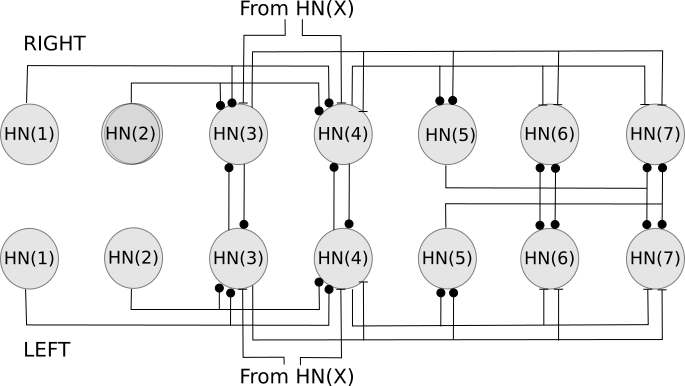
\includegraphics[width=\columnwidth]{graphics/leech.png}
		\caption[The Leech Heartbeat.]{\textbf{The Leech Heartbeat.} A network diagram of the leech heartbeat \ac{CPG} showing known synaptic connections between heart inter-neurons. HN(1) to HN(7) are the identified inter-neuron pairs while HN(X) is the unidentified neuron pair. All synapses are inhibitory except for the connections from HN(X) to HN(3) and HN(4). Adapted from \cite{Calabrese1977}.}
		\label{fig:leech}
\end{figure}


\subsection{\species{Tritonia}}
\species{Tritonia} is a gastropod mollusc. The swim \ac{CPG} of \species{Tritonia} has been a model system for studying rhythmic motor pattern generation for many years. The \species{Tritonia} swim \ac{CPG} is also a  network oscillator in that it has no neurons with intrinsic burst properties. Rhythmic bursting arise through conventional synaptic interactions. This \ac{CPG} is initiated by sensory input which results from contact with the tube feet of certain predatory sea stars \cite{Getting1985}.

The swim \ac{CPG} consists of the \ac{C2}, the \ac{DSI} and two types of \acp{VSI}. In a basic scenario the swim motor pattern is initiated by sensory input that activates \ac{DRI}. \ac{DRI} excites \ac{DSI} which, in turn, excites \ac{C2}. \ac{C2} feeds back and excites \ac{DRI}, which then further excites \ac{DSI} via a positive feedback loop. \ac{C2} excites \acp{VSI}, which then inhibits \ac{DSI} and \ac{C2}, thus momentarily interrupting the positive feedback loop. Figure \ref{fig:Tritonia_swim_CPGcircuit} shows the \species{Tritonia} swim \ac{CPG} circuit. The figure also shows the S-cells which are both mechanoreceptive and chemoreceptive. Excitaton of the S-cells are conveyed onto the Tr1 and \ac{DRI} cells via excitatory glutamatergic synapses \cite{Frost1996, Katz2009}).

\begin{figure}[H]
	\centering
	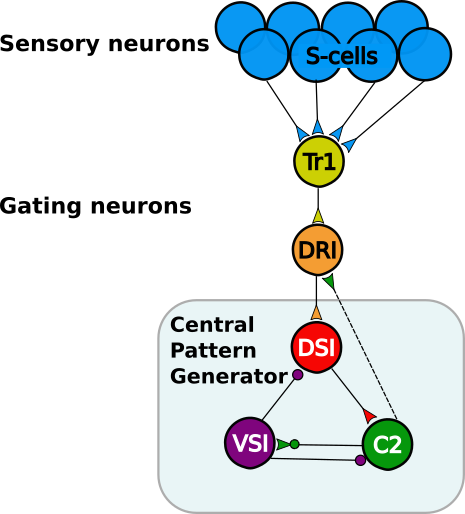
\includegraphics[width=9cm]{graphics/Tritonia_swim_CPGcircuit.png}
	\caption[The \species{Tritonia} swim \ac{CPG}.]{\textbf{The \species{Tritonia} swim \ac{CPG}}. This circuit shows the synapses involved in the  Circles represent inhibitory synapses and triangles represent excitatory synapses. Combinations of circles and triangles represent multicomponent synapses. (Adapted from \cite{Katz2009})}
	\label{fig:Tritonia_swim_CPGcircuit}
\end{figure}

The \acp{DSI} not only activate \ac{C2} synaptically but also via neuromodulation. Both the synaptic and neuromodulatory activation are mediated by serotonin (5-HT), which is released by the \ac{DSI} \cite{Katz1995, Katz1997}.

Some of the neurons in the swim \ac{CPG} of \species{Tritonia} have been found to be multi-functional in that they have functions other than just being involved in swimming. The \acp{DSI}, for example, excite neurons in the pedal ganglia that increase the speed of crawling \cite{Popescu2002}. Getting and Dekin used \species{Tritonia} as an example of a "polymorphic network" \cite{Getting1985a}.

\subsection{\species{Lymnaea}}
Yet another model organism which provides us with two more interesting \ac{CPG} networks for study is \species{Lymnaea stagnalis}, the pond snail. These \acp{CPG} are found in the feeding (see figure \ref{fig:Lymnaea_feeding_network}) and respiratory networks (see figure \ref{fig:Lymnaea_respiratory_network})  \cite{Kemenes2009}.

The name of \species{Lymnaea stagnalis} is deduced from the fact that it lives in stagnant water. The stagnant water leads to a hypoxic environment at which causes the snails to surface and perform rhythmic opening and closing movement of the pneumostome (the pulmonary opening). These movements are controlled by the respiratory \ac{CPG} \cite{Benjamin2008}. The \ac{RPeD1} initiates the respiratory rhythm while the \ac{IP3} causes the pneumostome to open (i.e. expiration) and the \ac{VD4} causes it to close (i.e. completion of inspiration). \ac{IP3} is connected to the I/J motoneuron via a monosynaptic excitatory connection. The activity of I/J causes the pneumostome to open. \ac{VD4} is connected to the K motoneuron, also via a monosynaptice excitatory connection. The activity of K causes the the pneumostome to close  \cite{Taylor2000}.

As in the case of \species{Tritionia} it has been found that many \species{Lymnaea} neurons are multifunctional \cite{Syed1991a, Kemenes2009}. For example, \ac{RPeD1}, a respiratory \ac{CPG} neuron has been found to co-ordinate sensory-motor input from the pneumostome at the water/air interface to initiate respiratory rhythm generation \cite{Haque2006}.

 \begin{figure}[H]
 	\centering
 	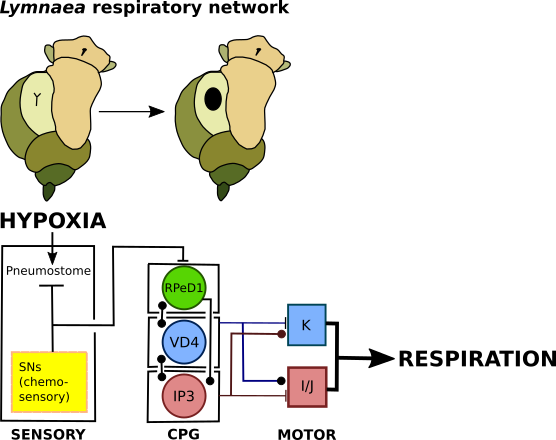
\includegraphics[width=\columnwidth]{graphics/lymnaea_b.png}
 	\caption[\species{Lymnaea respiratory network}]{\textbf{The \species{Lymnaea} respiratory \acp{CPG}}. The filled circles are inhibitory chemical synapses while the vertical bars indicate excitatory chemical synapses. Hypoxic conditions in stagnant water evokes compensatory changes in respiration. The \ac{CPG} consists of three neurons: 1) the \ac{RPeD1} which initiates the respiratory rhythm, 2) the \ac{IP3} which causes the pneumostome, via an excitatory monosynaptic connection to I/J, to open and 3) the \ac{VD4} which causes the pneumostome to close via the excitatory monosynaptic connection to K. (Adapted from \cite{Benjamin2008})}
 	\label{fig:Lymnaea_respiratory_network}
 \end{figure}
 
\species{Lymnaea} possesses a toothed radula which is used for feeding. Feeding consist of the mouth begin opened and the radula being scraped over the food substrate. The food is lifted into the mouth and the mouth is then closed while the food is swallowed. These movements are repeated while the snail is feeding. The rhythmic movements of the feeding muscles are driven by motorneurons which in turn are driven by synaptic inputs from the feeding \ac{CPG}.

The \ac{CPG} interneurons are divided into three main classes, N1, N2, and N3. The classification is made according to the phase of the feeding pattern, i.e. protraction, rasp (or retraction) and swallow. These neurons provide  sequences of excitatory and inhibitory synaptic inputs to motorneurons involved in the three phasic feeding rhythm. The rhythmic activity of the \ac{CPG} relies on both synaptic connections and intrinsic electrical properties of the N neurons \cite{Vavoulis2007}. Activity in the \ac{CPG} neurons and in the motoneurons are modulated by higher order interneurons such as the \ac{CGC}, \ac{SO} and \ac{CBI}. 

The frequency of the feeding \ac{CPG} is controlled by the \ac{SO} via know synaptic connectivity. The \ac{SO} is extrinisic to the \ac{CPG}. The rhythm is driven by a steady depolorisation of the N1 cells. Brief stimulation of N2 and N3 resets the phase of the rhythm. The N1 neurons excite the N2 interneurons which in turn inhibit the N1 cells \cite{Elliott1985}.

 \begin{figure}[H]
 	\centering
 	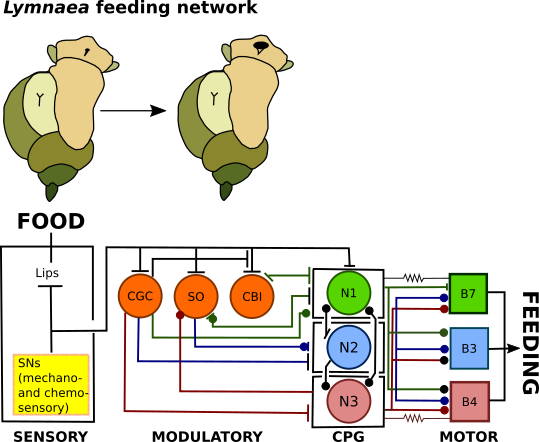
\includegraphics[width=\columnwidth]{graphics/lymnaea_a.png}
 	\caption[\species{Lymnaea feeding network}]{\textbf{The \species{Lymnaea} feeding \acp{CPG}}. The filled circles are inhibitory chemical synapses while the vertical bars indicate excitatory chemical synapses. Resistor symbols indicate electrical synapses. B7, B3 and B4 are motoneurons. Neurons N1, N2 and N3 form the \ac{CPG}. B7, B3 and B4 are motoneurons. The activity of all these neurons are modulated by higher order neurons such as the \ac{CGC}, \ac{SO} and \ac{CBI}. (Adapted from \cite{Benjamin2008})}
 	\label{fig:Lymnaea_feeding_network}
 \end{figure}

\section{The Crustacean Stomatogastric Nervous System}
The model system chosen for this research was the previously mentioned pyloric network found in the \ac{STG} which is located in the \ac{STNS} of crustaceans. In the case of the \ac{STG}, forming hypothesis of processes in more complex systems can be done by demonstrating in detail how cellular infrastructure produces rhythmicity and specialised patterns \cite{Selverston2010}.

The \ac{STNS} has been a tool for research into neural circuit dynamics for more than 40 years and a number of different crustacean species have been employed. These species include spiny lobsters (\species{Panulirus argus} and \species{Panulirus interruptus}), clawed lobsters (\species{Homarus americanus} and \species{Homarus gammarus}), various crab species (\species{Cancer borealis} and \species{Cancer pagurus}), crayfish and shrimp \cite{Marder2007}.

A detailed description of the gross anatomy of the stomatogastric system is beyond the scope of this thesis. There is, however, an extensive literature available on this subject, of which the writings of Selverston, Maynard and Dando \cite{Selverston1976,Maynard1973} are probably the most prominent.

In crustaceans the \ac{STNS} (Fig: \ref{fig:location_STNS} and \ref{fig:STNS}) is an extension of the central nervous system, controlling the foregut by innervating the striated muscles that produce rhythmic movement in the oesophagus, cardiac sac, gastric teeth and the pyloric chamber \cite{Selverston1987}. It consists of four ganglia: the \ac{OG}; the paired \acp{CoG}; and the \ac{STG}. The \ac{OG} contains about 18 neurons, while each of the \acp{CoG} contains about 400 neurons \cite{Marder2007}.

\begin{figure}[H]
	\centering
		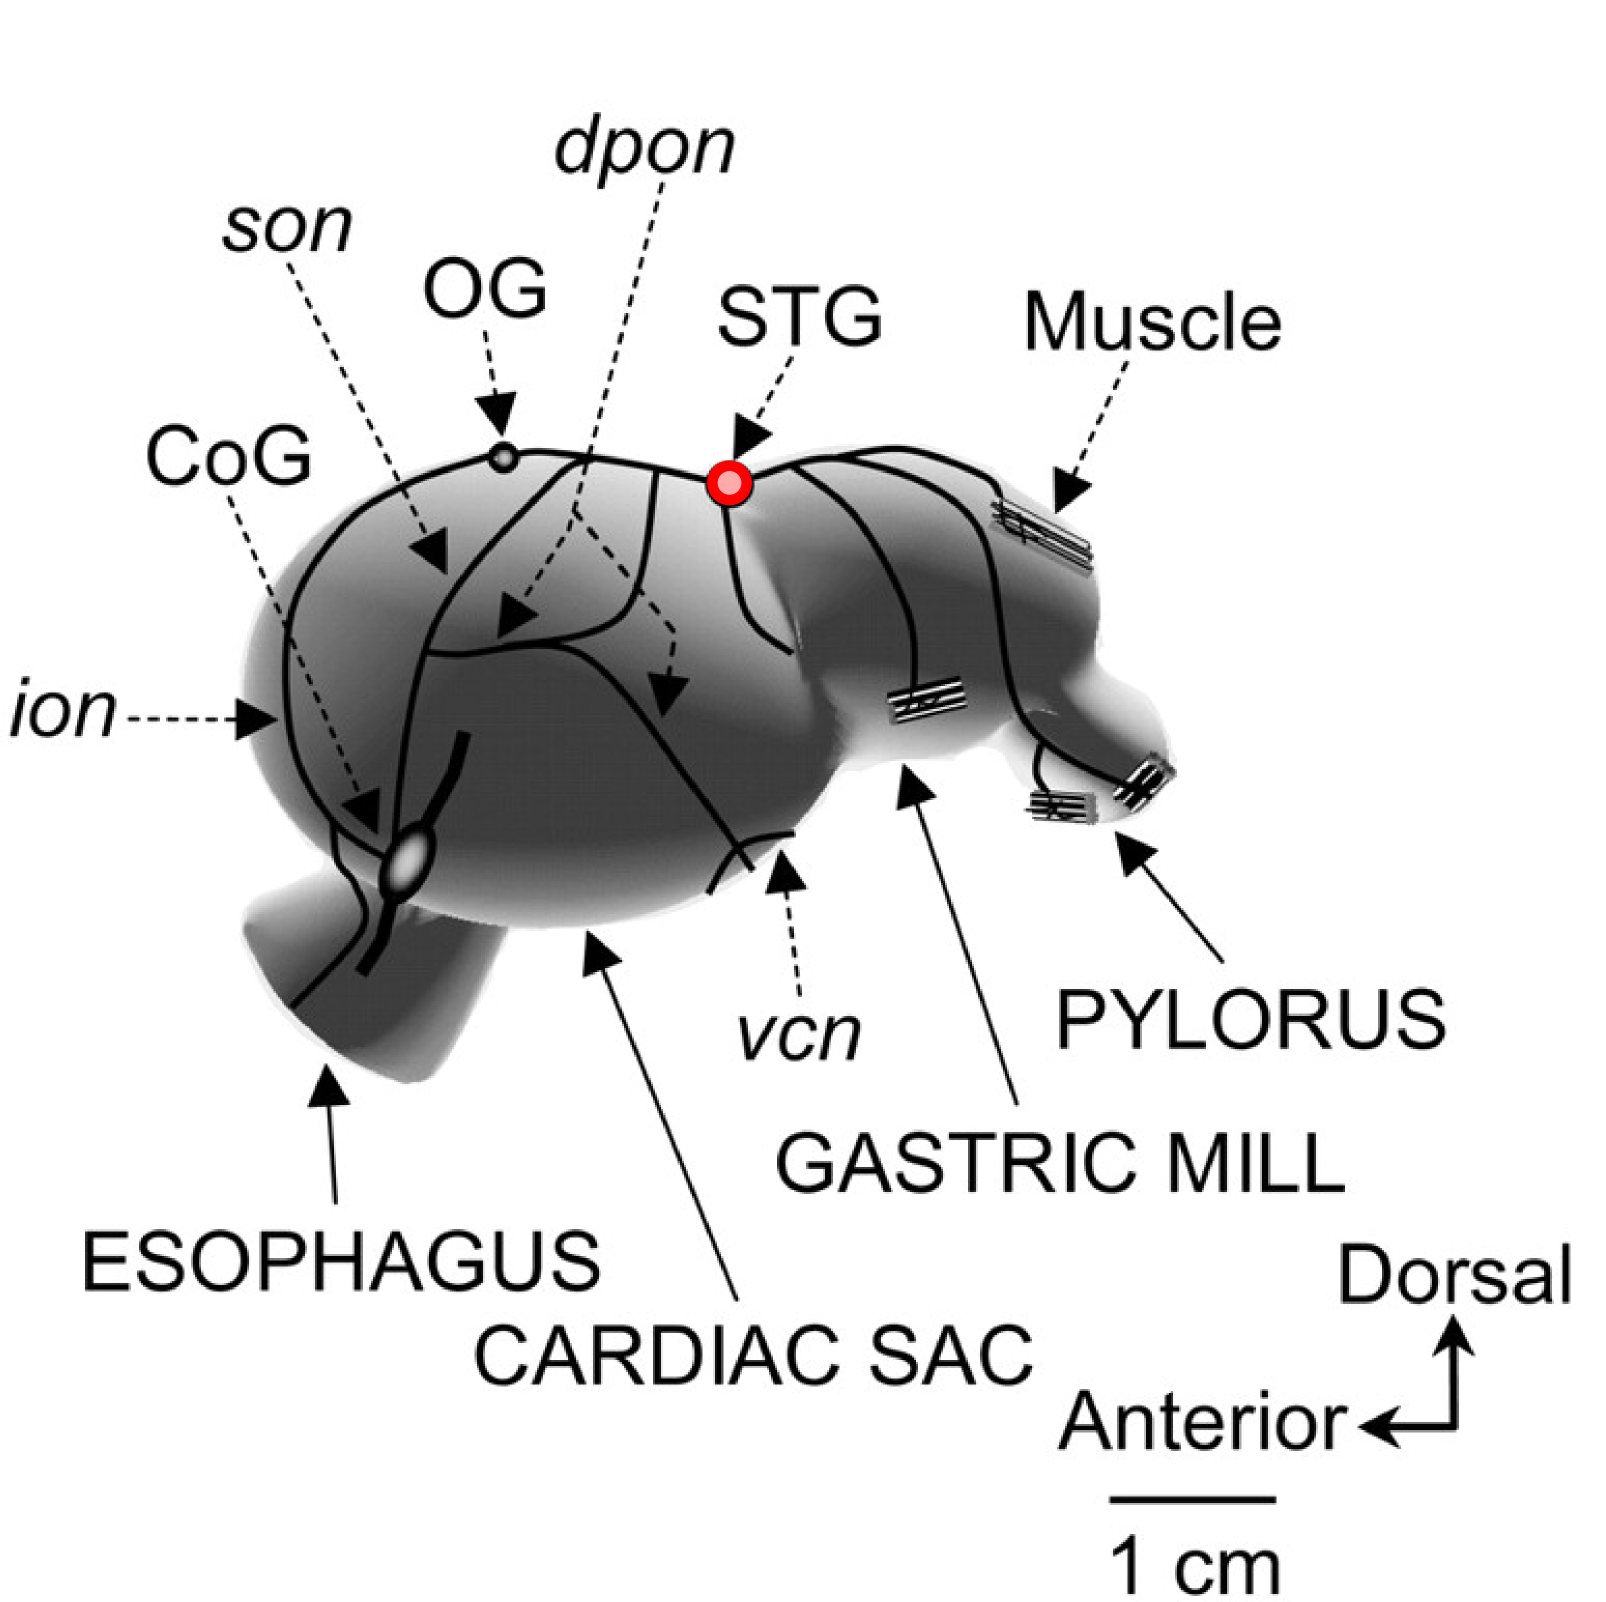
\includegraphics[width=9cm]{graphics/foregut_stns_beenhakker.png}
		\caption[Location of the crab \ac{STNS} around the stomach.]{\textbf{Location of the crab \ac{STNS} around the stomach.} Shown is the innervating \ac{STNS}, in black, and the \ac{STG}, in red, around the crab foregut. Arrows with dotted lines point to \ac{STNS} elements which include the \ac{ion}, \ac{CoG}, \ac{son}, \ac{OG}, \ac{dpon}, \ac{STG}, a muscle and the \ac{vcn}. Arrows with solid lines point to foregut regions (Adapted from \cite{Beenhakker2004})} 
		\label{fig:location_STNS}
\end{figure}

The underlying circuitry of the \ac{STNS} is well known. Figure \ref{fig:stns_connectome} shows the pyloric and gastric circuits that comprise the lobster stomatogastric nervous system.

\begin{figure}[H]
	\centering
		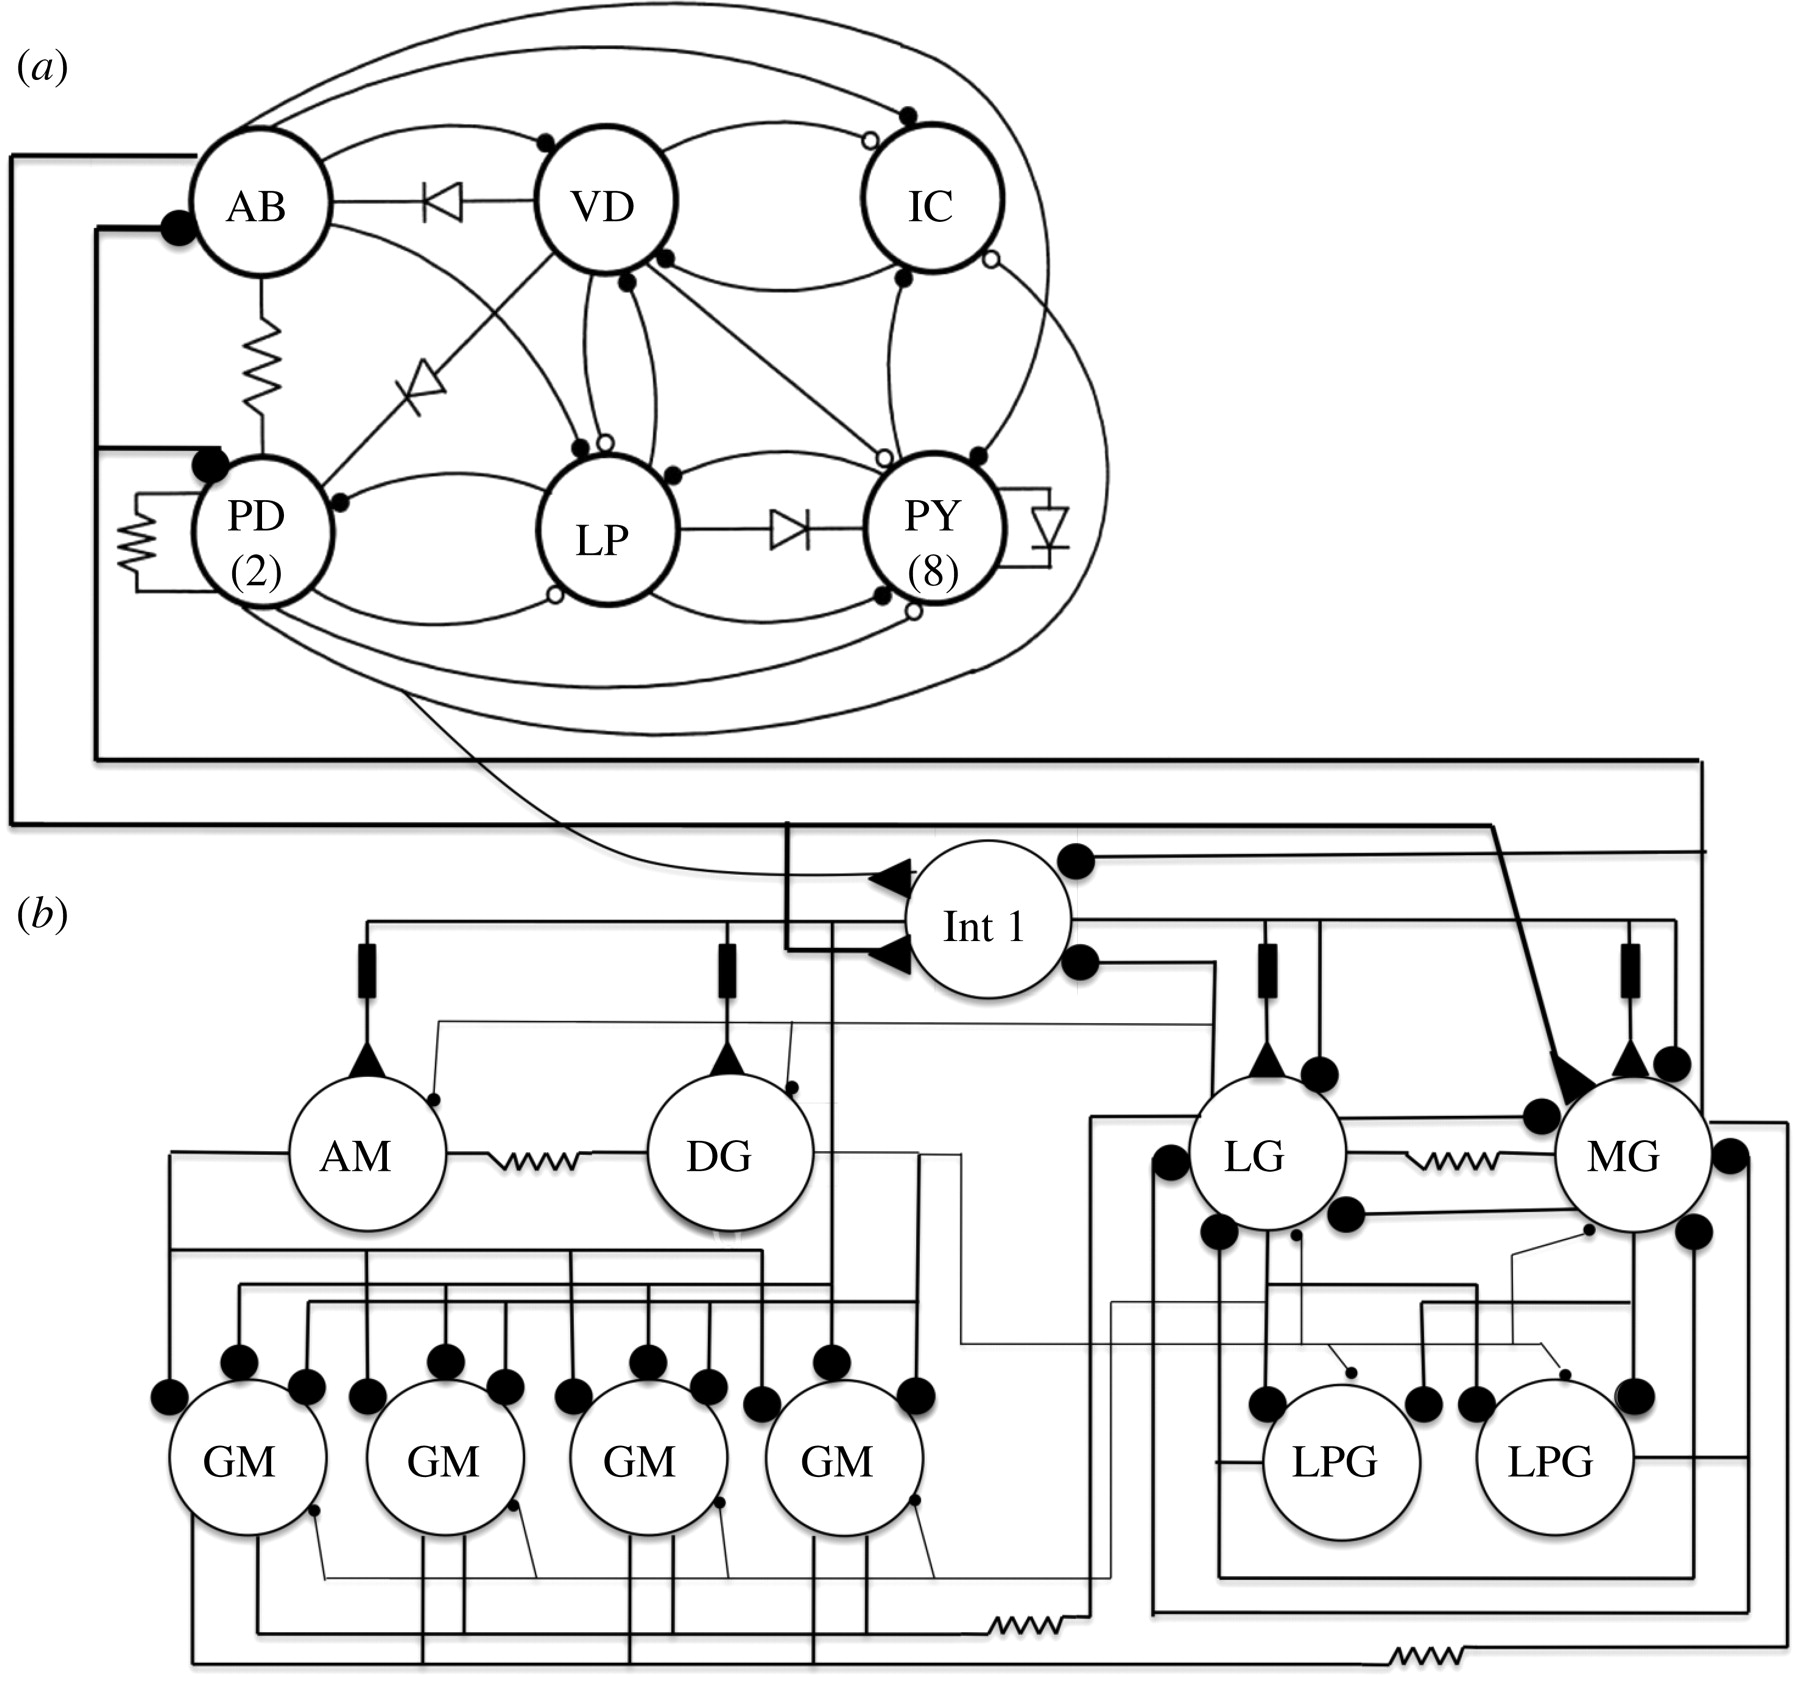
\includegraphics[width=\columnwidth]{graphics/stns_connectome.png}
		\caption[The underlying circuitry of the lobster stomatogastric network.]{\textbf{The underlying circuitry of the lobster stomatogastric network.} Symbols: large circles, neurons; black dots, inhibitory synapses; triangles, excitatory synapses; resistors, electrical coupling and diode symbols,  rectifying electrotonic connections. The rectangles represent delay lines between spikes in the presynaptic neurons and postsynaptic excitatory repsonse. Adapted from \cite{Selverston2010}}
		\label{fig:stns_connectome}
\end{figure}

\begin{figure}[H]
	\centering
		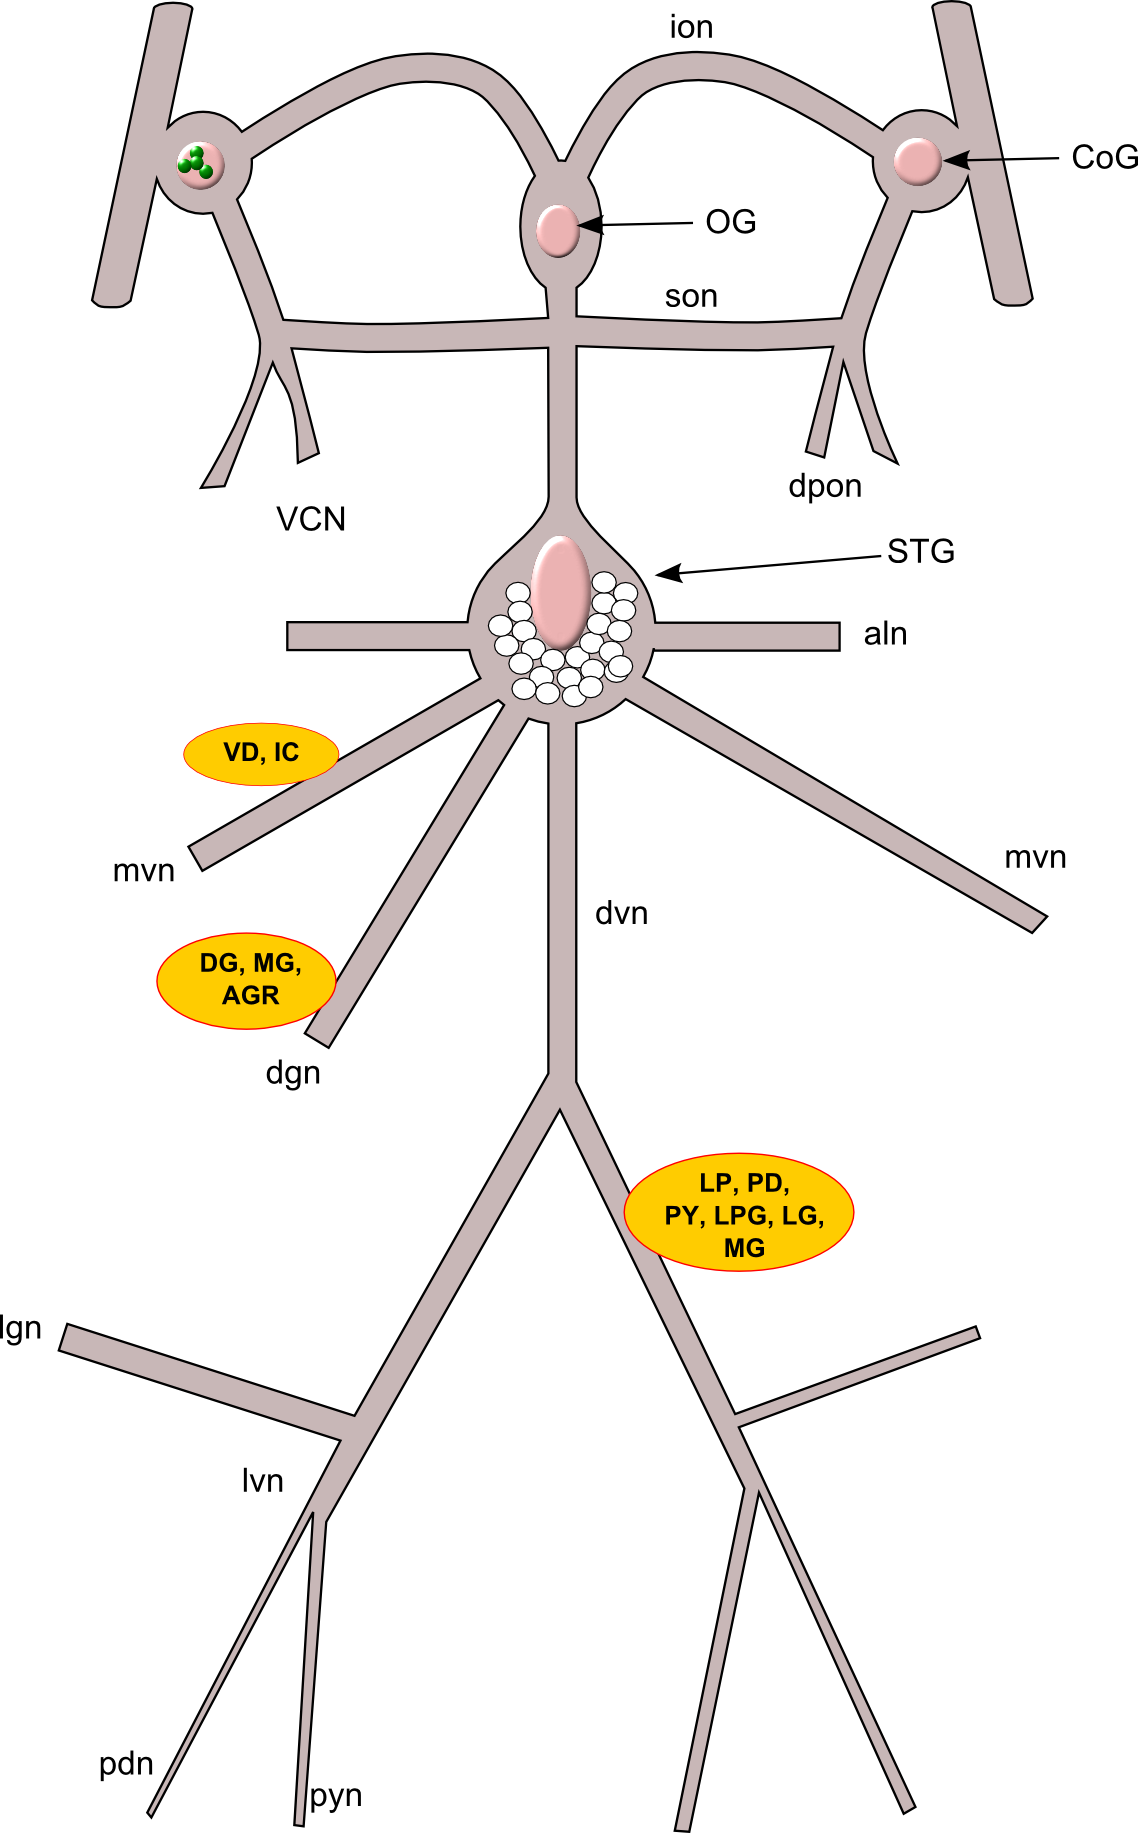
\includegraphics[width=9cm]{graphics/STNS.png}
		\caption[The stomatogastric ganglion.]{\textbf{The Stomatogastric Ganlgion.} A diagram of the stomatogastric nervous system (STNS) showing the commisural ganglia (CoG), the oesophageal ganglion (OG), the \ac{STG} (STG) and all interconnecting nerves (ion, son, dpon, stn, vcn, aln, mvn, dgn, dvn, lgn, lvn, pdn, pyn). Lower case abbreviations are used for the nerves while capitalised abbreviations are used for neurons. All neurons (AB, AM, AGR, DG, GM, Int1, LG, LP, LPG, PD, MG, PY, VD) are located in the stomatogastric ganglion (STG). The axons of neurons projecting down specific nerves are shown in the orange circles. }
		\label{fig:STNS}
\end{figure}

\section{The Stomatogastric Ganglion}

The \ac{STG} is found on the dorsal surface of the foregut of decapod crustaceans (Fig: \ref{fig:location_STNS}). The ganglion consists of 24-26 neurons in crabs and 29-32 neurons in lobsters. These neurons form two \acp{CPG}, the pyloric and gastric mill \acp{CPG}. Differences in the number of \acp{GM} and \acp{PY} between species account for the variability in the number of neurons \cite{Marder2007}.

\begin{figure}[H]
	\centering
		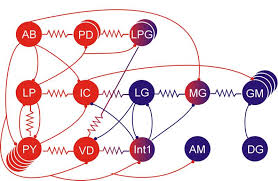
\includegraphics[width=\columnwidth]{graphics/stg.jpg}
		\caption[Neurons of the stomatogastric ganglion.]{\textbf{Neurons of the stomatogastric ganglion} with all inhibitory and electrical synapses indicated. Inhibitory synapses are shown as circles on the neuron that is inhibited. Electrical synapses are indicated by the resistor symbol (a zig-zag). The circuit consists of one \acf{AB}, two \acfp{PD}, two \acfp{LPG}, one \acf{LP}, one \acf{IC}, one \acf{MG}, four \acfp{GM}, five \acfp{PY} (which could vary between four and eight depending on the species), one \acf{VD}, one \acf{Int1}, one \acf{AM} and one \acf{DG}. (from \url{http://www.bio.brandeis.edu/marderlab//figures/circuit.jpg})}
		\label{fig:STG}
\end{figure}


The pyloric \ac{CPG} produces a cyclic three-phase rhythm that controls the striated muscles which constrict and dilate the pyloric region of the stomach. The pyloric region is a section of the foregut that is responsible for the filtering of masticated food. Chewing is controlled by a six-phase rhythm produced by the gastric mill \ac{CPG} \cite{Marder2001, Selverston2005, Selverston2010}, controlling the movements of two lateral teeth and one medial tooth \cite{Heinzel1993}.

However, these two rhythms are not the only output that can be generated by the \ac{STG}. The networks in the \ac{STG} are very plastic and can be reconfigured by neuromodulation to produce multiple variants of the basic rhythms. The neurons of the two \acp{CPG} can even be recruited into other motor networks \cite{Johnson2003, Nusbaum2002}.


\subsection{Neurons of the STG}
The gastric \ac{CPG} is comprised of 11 neurons. Eleven to 14 of the neurons in the \ac{STG} belong to the pyloric \ac{CPG}. The number of neurons in the pyloric \ac{CPG} varies between species and between individuals within a species \cite{Daur2012a}. The lobster (\textit{Homarus americanus}), for instance, has eight PY neurons while the crab (\textit{Cancer pagurus}) has only four or five. Compared to mammalian neurons, the neurons of the \ac{STG} have relatively large somas of 50 to 100$\mu$m in diameter \cite{Marder2007}.

Both chemical and electrical synapses are found in the \ac{STG}. All of the chemical synapses are inhibitory \cite{Selverston1987}, with the exception of those involving projection neurons. The projection neurons are located in the \acp{OG}, projecting axons down the \ac{stn} to the \ac{STG}. The \ac{STG} neurons are mostly motor neurons and make excitatory neuromuscular connections \cite{Marder1987}.

Tables \ref{tab:gastric} and \ref{tab:pyloric} give the number of each neuron, its name, abbreviation and the muscle it innervates for the gastric and pyloric \acp{CPG} respectively. The abbreviations used for the neurons, nerves and muscles are based on a convention created by Maynard and Dando in which the nerves are named after the muscle they innervate \cite{Maynard1973, Marder1979a}.

\renewcommand{\tablename}{Table}
\begin{table}
	\centering
	\caption[Neurons of the Gastric \ac{CPG}]{\textbf{Neurons of the Gastric \ac{CPG}}}
	\label{tab:gastric}
	\begin{tabular}{l l l l }
		\hline
		\bf \# & \bf Neuron name & \bf Abbr. & \bf Muscle\\ \hline
		1 & Interneuron 1 & (Int 1) & interneuron \\ 
		4 & Gastric Mill & (GM) & gm 1, 2a, b \\ 
		1 & Dorsal Gastric & (DG) & gm 4a, b, c \\ 
		1 & Anterior Median & (AM) & c6, c7 \\ 
		1 & Lateral Gastric & (LG) & gm 5b, 6a \\ 
		1 & Medial Gastric & (MG) & gm 9a, 9c \\ 
		2 & Lateral Posterior Gastric & (LPG) & gm 3 \\ 
		\hline
	\end{tabular}
\end{table}

\begin{table}
	\centering
	\caption[Neurons of the Pyloric \ac{CPG}]{\textbf{Neurons of the Pyloric \ac{CPG}}}
	\label{tab:pyloric}
	\begin{tabular}{l l l l}
		\hline
		\bf \# & \bf Neuron name & \bf Abbr. & \bf Muscle\\ \hline
		1 & Anterior Burster & (AB) & inter-neuron \\ 
		2 & Pyloric Dilator & (PD) & cpv 1 and 2 \\ 
		1 & Lateral Pyloric & (LP) & p1 \\ 
		1 & Ventricular Dilator & (VD) & cv2 \\ 
		1 & Inferior Cardiac & (IC) & cv3 \\ 
		4 - 8 & Pyloric Constrictor & (PY) & p2-4, 7-9, 1-11 \\ 
		\hline
	\end{tabular}
\end{table}

Both these \acp{CPG}
produce rhythms that can be recorded intracellularly and extracellularly. In both cases the recordings obtained from \textit{in vitro} preparations are largely indistinguishable from those obtained from intact crabs  (figure \ref{fig:pyloric_rhythm_in_vivo_in_vitro}) \cite{Hedrich2011}.

\begin{figure}[H]
	\centering
		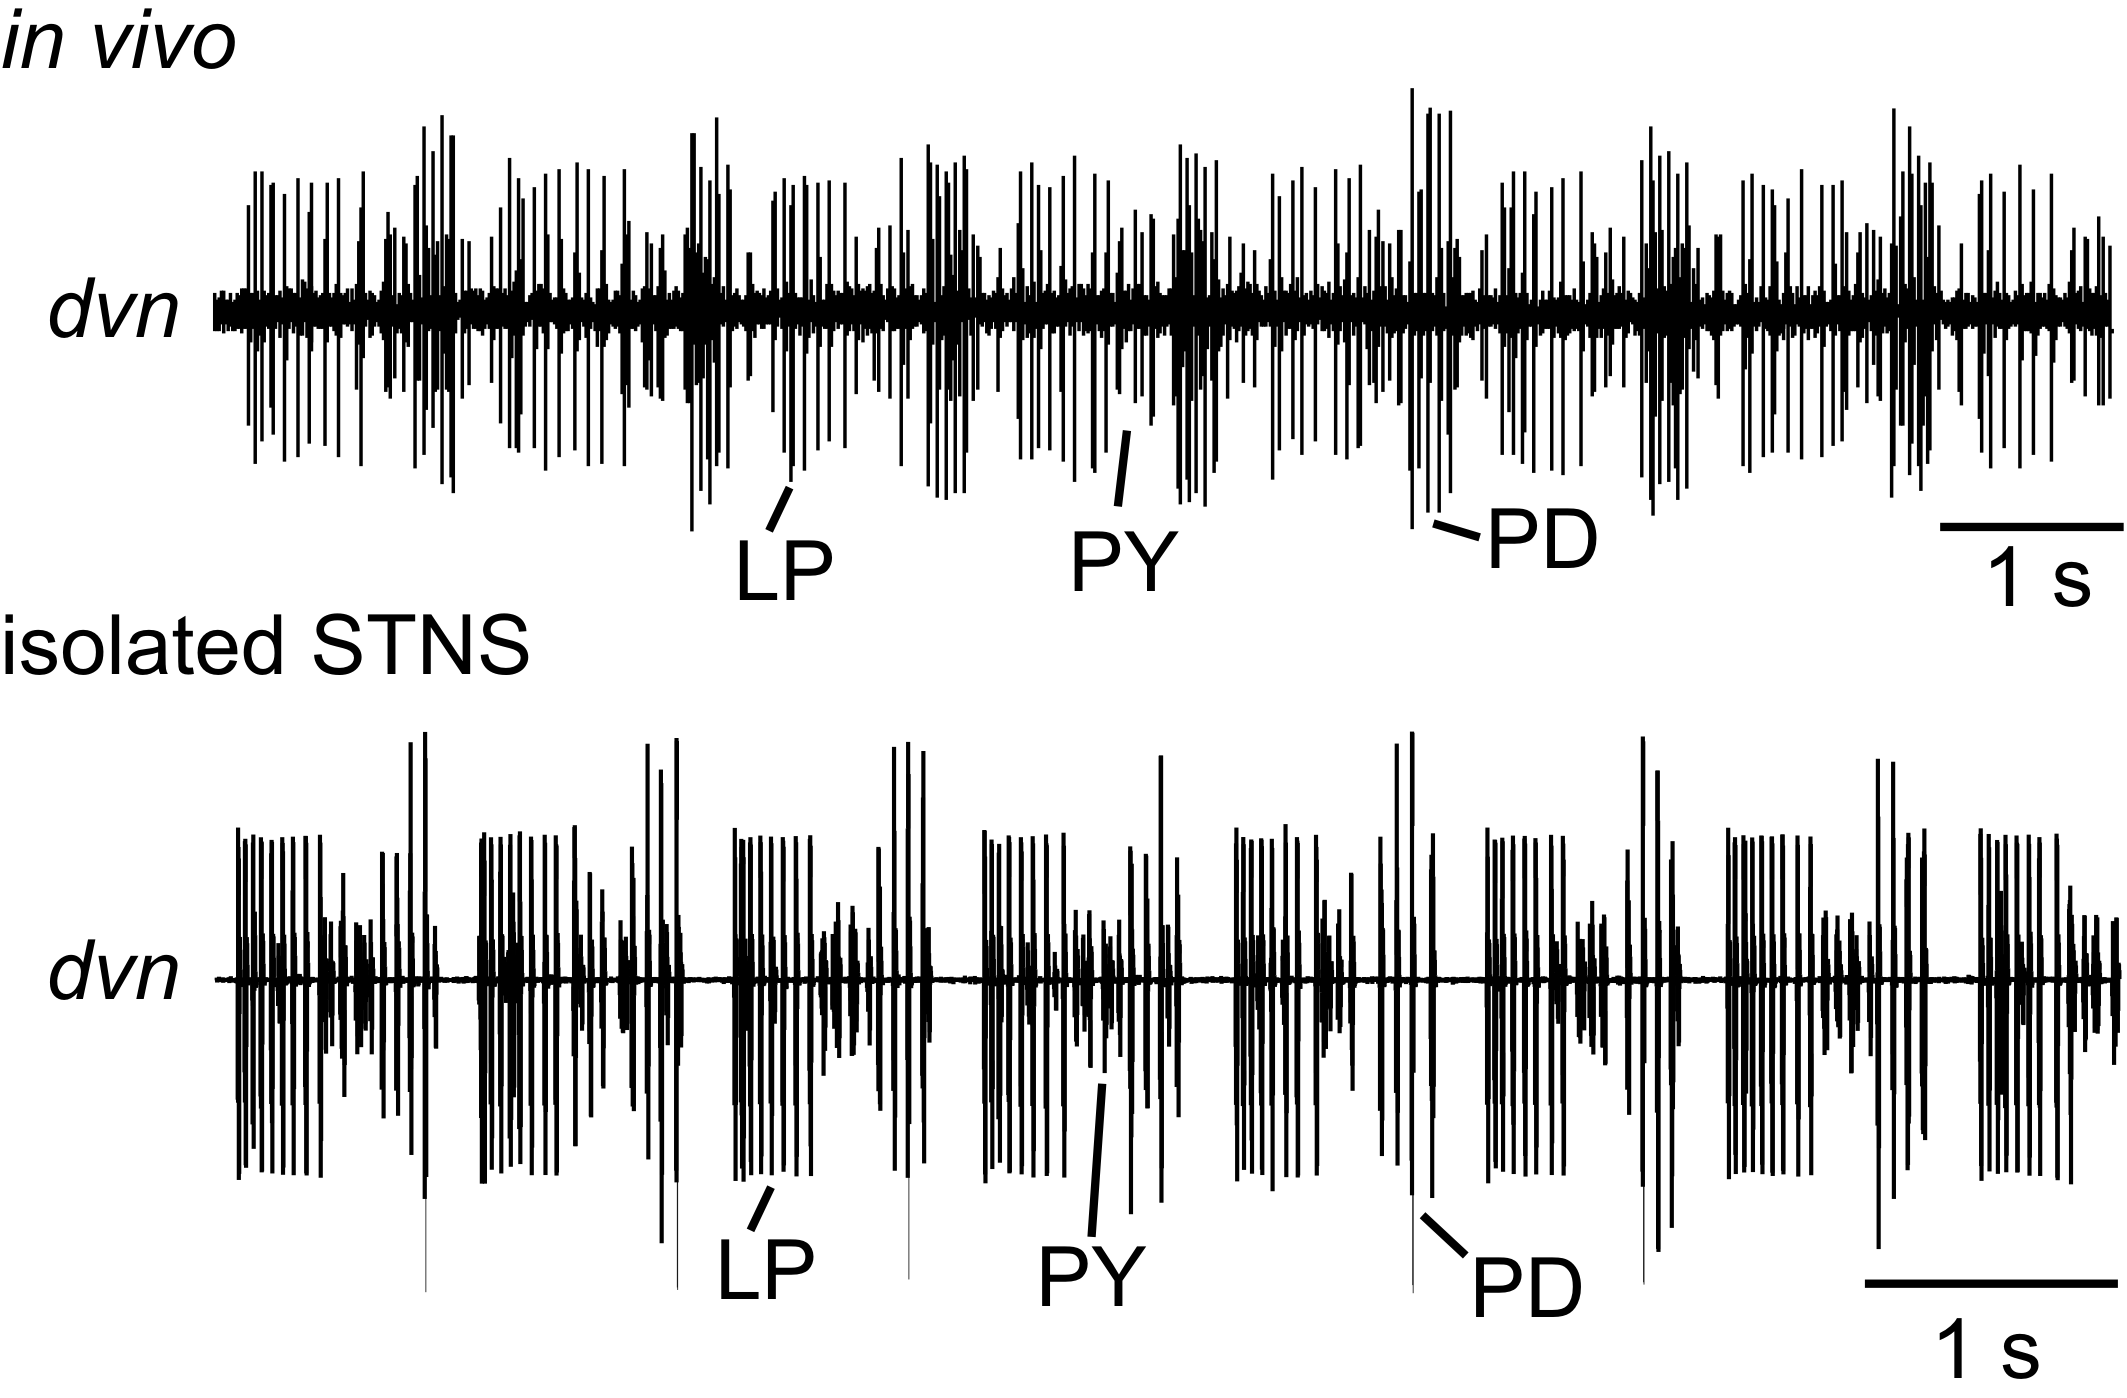
\includegraphics[width=8.5cm]{graphics/pyloric_rhythm_in_vivo_in_vitro.png}
		\caption[In vivo and in situ recordings of gastric and pyloric neurons]{\textbf{In vivo and in situ recordings of gastric and pyloric neurons} over the \ac{dvn} and \ac{mvn} in \species{Cancer borealis}. The recordings are largely indistinguishable. Adapted from \cite{Hedrich2011}, courtesy of Wolfgang Stein.} 
		\label{fig:pyloric_rhythm_in_vivo_in_vitro}
\end{figure}

%Weimann 1991
%Katz 1991

\subsection{Neurons of the Pyloric CPG}

Interneurons are neurons that form connections between other neurons while motor neurons carry signals to the muscles to produce movement. Motor neurons interface with muscles through specialised synapses known as neuromuscular junctions. Of the 11 to 14 neurons of the pyloric \ac{CPG} one is an inter-neuron, the \ac{AB}, while the rest, the \acp{PD}, \ac{LP}, \acp{PY}, \ac{VD} and \ac{IC} are motor neurons. 

% Buchholtz1992 - more about LP
%================================
There are two major classes of bursting neurons. Firstly there are constitutive bursters which rely on ionic conductances for its bursting. The second class of bursting neurons are the conditional bursters which rely on ionic mechanisms to generate rhythmic activity. 
%\when isolated these cells loose the ability to burst. Harris-Warrick1987

The \ac{AB} is an endogenous oscillator which can oscillate even when isolated from the network. The \ac{AB} is electrically connected to the \acp{PD} via gap junctions \cite{Zhao2010} to form what is known as the pacemaker group. The \ac{AB} oscillates, in conjunction with the \acp{PD}, to serve as a kernel pacemaker that drives the pyloric circuit at a rate of approximately one Hertz \cite{Soto-Trevino2005, Abbott1991}. This pacemaker group acts as the timer for pyloric rhythm. Typical of pacemaker-driven activity, the depolarisation of the \ac{AB} increases the frequency of bursting while depolarisation decreases the frequency \cite{Selverston1985}. Together the \ac{AB} and \acp{PD} inhibit the \acp{LP} and \acp{PY}. This inhibition forces the \acp{LP} and \acp{PY} to fire alternately with the \acp{PD} \cite{Bargmann2013}. The \acp{PY} take longer to rebound from inhibition than the \acp{LP}, and are therefore inhibited further by the \acp{LP}. When the \acp{PY} do rebound from inhibition they terminate the \acp{LP} \cite{Marder2007}.

The \acp{PD} drive one muscle group of the pylorus. The  \ac{LP} and \ac{PY} follower neurons drive another group of muscles. Fig. \ref{fig:pyloriccpg} shows the neurons of the pyloric \ac{CPG} and their connections with one another.

Bursting in neurons is produced by a combination of slow inward currents that produce a depolarising phase followed by activation of a slow outward current that terminates the burst. There are also faster, voltage-gated currents, which account for spikes during the depolarised phase allowing action potentials and bursting to co-exist. It has been hypothesised that Ca\textsuperscript{2+} is part of the inward current. Ca\textsuperscript{2+} accumulation activates the Ca\textsuperscript{2+}-activated K\textsuperscript{+} currents that have been shown to terminate bursts in several systems \cite{Levi2003} %check Amini et al. 1999; Kiehn and Harris Warrick, 1992



\begin{figure}[H]
	\centering
		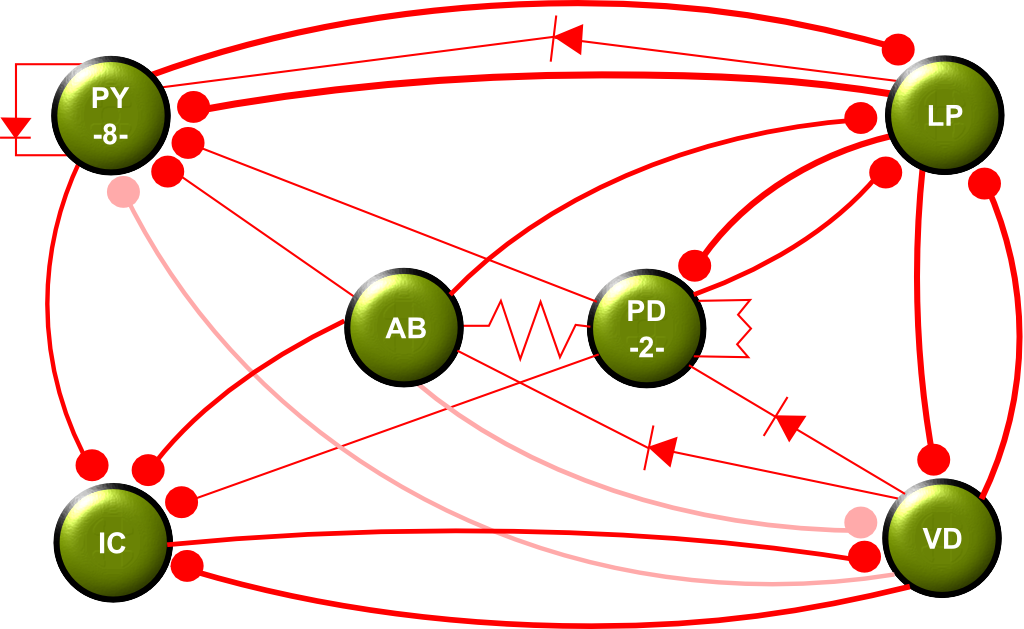
\includegraphics[width=9cm]{graphics/pyloriccpg.png}
		\caption[Neurons of the pyloric \ac{CPG}.]{\textbf{Neurons of the pyloric \ac{CPG}.} Inhibitory synapses are shown with filled circles; non-rectifying electrical synapses are shown with a resistor and rectifying synapses are shown with a diode symbol that also shows the direction of the preferred current flow. (Adapted from \cite{Harris-Warrick2011})}
		\label{fig:pyloriccpg}
\end{figure}

\subsection{Neurons of the Gastric Mill CPG}
The gastric mill \ac{CPG} also has one inter-neuron, \ac{Int1}, while the remaining neurons, the \acp{GM}, \ac{DG}, \ac{AM}, \ac{LG}, \ac{MG} and \acp{LPG} are motor neurons. The gastric mill \ac{CPG} produces a five-phased motor pattern. Chemical synapses in this \ac{CPG} are inhibitory, while electrical synapses are mostly non-rectifying. The \ac{LG} and \ac{MG} neurons fire at about the same time, and alternate with the \ac{LPG}. The \ac{DG}, \ac{AM} and \ac{Int1} fire together and alternate with the \ac{GM} \cite{Harris-Warrick1992}.

\begin{figure}[H]
	\centering
		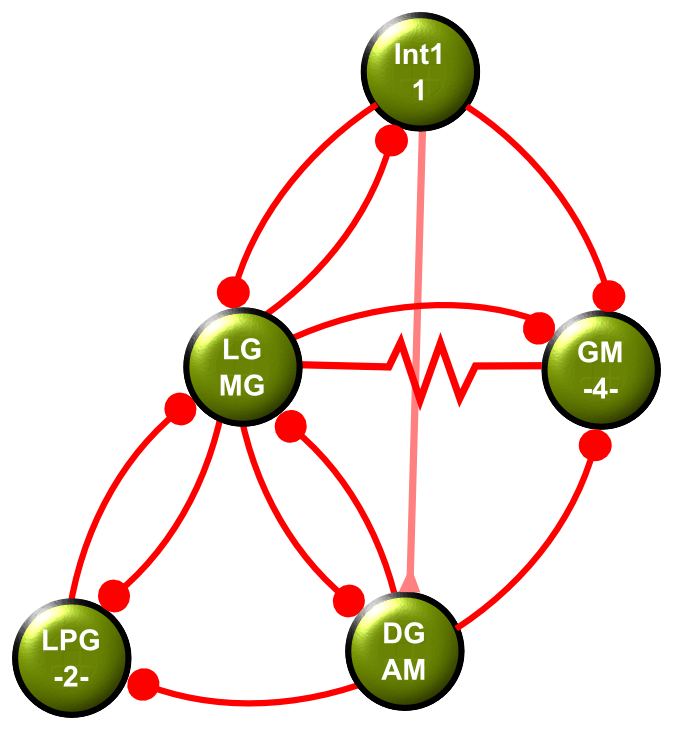
\includegraphics[width=9cm]{graphics/gastriccpg.png}
		\caption[Neurons of the gastric mill \ac{CPG}.]{\textbf{Neurons of the gastric mill \ac{CPG}}.  Inhibitory synapses are shown with filled circles; non-rectifying electrical synapses are shown with a resistor, (Adapted from \cite{Harris-Warrick1992})}
		\label{fig:gastriccpg}
\end{figure}

In crustacea, the gastric mill \ac{CPG} controls the chewing movements of three teeth located in the gastric mill \cite{Rowat1993}.

\section{Neuromodulation}
\note{ NEUROMODULATORS  CAN  ALTER  SYNAPTIC EFFICACY Harris-Warrick1991}
Despite the fact that the complete ``wiring diagram'' for the \ac{STG} has been known for more than 25 years, it was soon clear that the static connectivity diagram could not capture the dynamics of the circuit \cite{Abbott1998}. An interesting phenomenon in neural systems is their ability to maintain stability despite environmental changes. These changes include extracellular conditions as well as channel turnover and cell growth \cite{LeMasson1993}.  Flexibility to cope with such changes is provided for by sensory input, neuromodulation which tunes the intrinsic neuronal excitability and synaptic properties of neurons as well as the inputs to the circuits of which the neurons are part \cite{Bucher2013, Johnson2005, Nadim2014}. 

Neuromodulation is caused by substances known as neuromodulators, such as amines, neuropeptides, gasses and small-molecule neurotransmitters. Some neuromodulators are produced locally by the neurons while others are released remotely and transferred to neurons through the bloodstream. These molecules are known as neurohormones \cite{Stein2009}. 

The source of neuromodulators in modulated circuits can be intrinsic or extrinsic. In the latter, the cells releasing the neuromodulators are not part of the modulated circuit. Indirect feedback to the neurons of origin might, however, exist. In the former the neurons releasing the neuromodulator are part of the modulated circuit \cite{Bucher2013}.

In the \ac{STNS} all stages of the neuronal processing are affected by factors such as membrane currents, synaptic transmissions, or the properties of the effector muscles \cite{Stein2009}. At least 18 neuromodulatory substances are found in the \ac{STG} \cite{Marder1987, Marder1995, Marder2001, Marder2007}, and the same neuromodulator can differently affect pyloric neurons \cite{Baro1997} (Table \ref{tab:neuromodulators}).

\begin{table}[htbp]
	\centering
	\caption[Secreted Amines and Neuropeptides of the \ac{STG}]{\textbf{Secreted Amines and Neuropeptides of the \ac{STG}}. At least 18 different neuromodulatory substances are found in the \ac{STG}.}
	\begin{tabular}{l l l}
		\hline \bf Modulators & \textbf{Neurohormones} & \textbf{Sensory Transmitters} \\\hline
		AST   & 5-HT  & ACh \\
		BUC   & OCT   & AST \\
		CCKC36-9H & DA    & 5-HT \\
		CCKC34-4E & CCAP  &  \\
		CCK223-R & PDH   &  \\
		CabTRP & AST   &  \\
		MYO   & BUC   &  \\
		PROC  & CCKC36-9H &  \\
		RPCH  & CCK234-4 &  \\
		FLRF  & GABA  &  \\
		ATR   & CabTRP &  \\
		Orcokinin & FLRF  &  \\
		ACh   & RPCH  &  \\
		DA    & PROC  &  \\
		GABA  & MYO   &  \\
		HA    & COR   &  \\
		OCT   & Orcokinin &  \\
		NO    &       &  \\
		\hline 
	\end{tabular}%
	\label{tab:neuromodulators}%
\end{table}%


\section{Dopamine}

\Ac{DA} is of interest to researchers because of the many functions it has in humans and animals. \Ac{DA} is associated with functions in attention, movement, memory, pleasurable reward, mood, learning and many more.

Conditions such as ADHD, addiction and schizophrenia are all associated with abnormal mid-brain dopamine levels \cite{Lammel2008}. Mesocortical \ac{DA} inputs to the \ac{PFC} regulates aspects of working memory and its dysfunctions underlie cognitive deficits associated with schizophrenia \cite{ Barch2012, Seamans2004, Slifstein2015}. It has been shown that adjunctive administration of \ac{DA} agonist can improve cognition in individuals with schizophrenia taking typical anti-psychotics \cite{Barch2005}.

Proper \ac{DA} actions in the \ac{PFC} is also of vital importance for the \ac{PFC} to mediate executive functions in goal directed behaviour \cite{Goto2007}. Several brain regions have been implicated in the control of motivated behaviour. Disruptions in any of these regions, eg. the ventral hippocampus, the amygdala, the \ac{PFC} and the limbic system, lead to the pathophysiology observed in several psychiatric disorders. What these brain areas have in common are overlapping projections to the nucleus accumbens, where the inputs are integrated under the modulatory influence of \ac{DA} \cite{Grace2007}.

\ac{DA} has been shown to be involved in regulating food intake by modulating food reward via the meso-limbic circuitry of the brain and thus associated with obesity and drug abuse \cite{Wang2001}.  It has been shown that the nucleus accumbens and dorsal striatum dopaminergic neurotransmission are depressed in obese rats and \ac{DA} levels can temporarily be restored by eating highly palatable, high-energy food \cite{Geiger2009}. This research has led to the hypothesis that individuals increase their reward seeking behaviour, which in this case is compulsive eating, as a mechanism to compensate for diminished \ac{DA} activity. A study by Jeff A. Beeler using \ac{D2R} knock-down mice, however, has shown that the primary contribution of altered \ac{D2R} signalling to obesity does not lie in the induction of compulsive eating but rather in altered energy expenditure. The knock-down mice used in Beeler's research exhibited significantly lower activity than wild-type mice \cite{Beeler2015}

The regulation of \ac{DA} has been associated with \ac{D2R} which are found in high density in the striatum, nucleus accumbens, the olfactory tubercle and to a lower extend in the hippocampus, amygdala, hypothalamus and cortical regions. These receptors play a key role in the regulation of dopaminergic neurons and are key in controlling the synthesis, release and uptake of \ac{DA}. \ac{D2R} are inhibitory and activation of \ac{D2R} decreases excitability of \ac{DA} neurons and the release of \ac{DA} \cite{Ford2014}.

Research such as the above-mentioned is usually done on mice and rats, using techniques such as carbon microfibre electrodes \cite{Suaud-Chagny1991}, retrograde tracers \cite{Root2014}, transgenic approaches and optogenetics \cite{Pignatelli2015} and involve whole brain regions. 

Also of interest is the association of \ac{DA} with neurodegenerative diseases such as Alzheimer's disease, \ac{PDis} and \ac{HD} disease. Of particular interest to this research is \ac{PDis} which is the second most common neurodegenrative disorder after Alzheimer's disease. \ac{PDis} is a degenerative disorder of the central nervous system which mainly affects motor systems and is caused by selective dopaminergic cell loss. The reasons for such cell loss is still not understood \cite{Lau2006}. 

Although there is only indirect evidence that \acp{CPG} exist in humans, it is generally accepted that locomotion is based on \acp{CPG} within the spinal cord \cite{Iosa2015}. Evidence is pointing to defective afferent input to \acp{CPG} being involved in movement disorders such as \ac{PDis}. It is thought that \acp{CPG} in humans are dispersed over several spinal segments. Conditions such as "Freezing of Gate" could be caused by disrupted descending control of these circuits and it has been shown that gait and turning abnormalities are more pronounced in \ac{PDis} patients when dopaminergic drugs are at their nadir, implicating dopaminergic contribution to freezing of gate \cite{Nutt2011}.

\subsection{\ac{DA} in the \ac{STG}}

\Ac{DA} acts in the \ac{STNS} both as a neurohormone and a neuromodulator \cite{Clark2008}. Neuromodulators are produced locally in the \acp{CoG} while neurohormones are produced elsewhere in the body and transferred to the \ac{STNS} via the blood \cite{Selverston1980a}. 

The \ac{STG} neurons do not, themselves, contain \ac{DA}, but because the \ac{STG} is located in the ophthalmic artery \cite{Claiborne1987} the neurons are always bathed in haemolymph, and thus receiving neurohormonal dopaminergic input. \ac{DA} is secreted into the haemolymph by the pericardial organs \cite{Clark2008}. \Ac{DA} has been shown to induce a distinct pyloric motor pattern when bath-applied to the \ac{STG} \cite{Johnson1990}.

\ac{DA} is one of the neuromodulators that can differentially modulate neurons in the pyloric network \cite{Clark2007}. Several changes to the pyloric motor pattern can be observed when \ac{DA} is applied. There are changes to the overall cycle frequency, the intensity of neural activity and the phases of the rhythm. The changes are the result of both alterations to the intrinsic properties of the cells and variations in the strength of synaptic interactions \cite{Harris-warrick1998}.

One of the effects that \ac{DA} has in the \ac{STG} is to excite some of the \acp{PY}, causing them to fire at a high frequency. In turn, the high frequency firing of the \acp{PY} cause a phase advance in the timing of the \acp{PY} relative to the pyloric rhythm \cite{Harris-Warrick1995}. The I$_A$ current is modulated in nearly every neuron of the pyloric network. Modulation, however, can be in opposite directions in different cells \cite{Harris-warrick1998, Baro1997}. The modulation of the I$_A$ current also affects the rate of post-inhibitory rebound and spike frequency of the \acp{PY}, which influences the pyloric cycle frequency and phase constancy \cite{Zhang2010}.

It has been shown, in lobsters, that modulation by dopamine can result in a significant increase in the input resistance of \ac{AB} and a simultaneous decrease in the input resistance of \ac{PD} \cite{Zhao2010}.

A further influence of \ac{DA} on the pyloric rhythm is the inhibition of the \ac{PD}s through the enhancement of I$_A$ and Ca-dependent outward current which in turn contributes to the reduction of spike frequency. The \ac{LP}, on the other hand, is excited through a decrease in I$_A$ and the enhancement of I$_h$. I$_h$ is a slow hyperpolarisation-activated inward current. \ac{DA} shifts the voltage activation curve for I$_h$ in a positive direction \cite{Harris-warrick1998}. Harris-Warrick \cite{Harris-warrick1998} has shown through modelling and dynamic clamp experiments that the reduction of I$_A$ is the predominant mechanism for \ac{DA} to excite the \ac{LP} neuron. The firing of the \ac{LP} and {PD} is regularised by \ac{DA} which, in turn, increases the reliability of recurrent spike patterns \cite{Szucs2005}.

Until recently not a great deal was known about the signalling events and molecular mechanisms that mediate the effects of \ac{DA}. However, the work of Deborah J. Baro has been filling this gap  \cite{Clark2007}. It has been shown that the G-proteins Gs, Gi and Gq are activated in response to \ac{DA} in the \ac{STNS} and that three evolutionary conserved \ac{DA} receptors were expressed to mediate the process. Research from this lab has also identified six Innexin proteins in \species{Cancer borealis} and \species{Homarus americanus}. It was shown that all the cells in the crab \ac{STG} express multiple innexin genes. Electrophysiological recordings also showed that the \ac{PD}-ac{PD} electrical synapse is non-rectifying while the \ac{PD}-\ac{LPG} synapse is strongly rectifying \cite{Shruti2014}.
\note{Oginsky2010,Clark2008} Understanding of the molecular mechanism is improving but still a lot of work needs to be done.

Johnson et. al. \cite{Johnson1993} investigated amine modulation of electrical coupling in the pyloric network and found that all the pyloric electrical synapses were modulated by \ac{DA}. The coupling strength of all the electrical synapses was either decreased or increased. They found that the \ac{AB} to \ac{PD} coupling was decreased when current was injected into \ac{AB}, but coupling in the other direction, \ac{PD} to \ac{AB}, increased. Furthermore \ac{DA} decreased \ac{AB} to \ac{VD} coupling when current was injected into either of the neurons. They also found that \ac{DA} increased the input resistance of the \ac{AB} neuron, but decreased the input resistance of the \ac{PD} and \ac{VD} neurons.


\section{Electrophysiology}

Electrophysiology is the study of the electrical properties of biological cells and tissues. More than 200 years ago Luigi Galvani not only paved the way for the invention of the electric battery but he also laid the foundations of electrophysiology \cite{Piccolino1997}. 

The mechanism underlying electric signalling in nerves became clearer with Hodgkin, Huxley and Katz's experiments with the squid giant axon in 1948 \cite{Huxley2002, Hodgkin1952}. The giant squid axon was used as a model system because it is unusually large and therefore very suitable for electrophysiological experiments. The voltage clamp method used in their experiments was devised by Cole and Curtis in the 1930s \cite{Cole1939}. 

Electrophysiology depends on three elements, time, voltage and current. The purpose of the voltage clamp is to eliminate one of these elements, voltage, to make it easier to study the changes in current over time. The voltage clamp works by using an internal recording electrode that is inserted into the axon and an external reference electrode to measure the voltage with an amplifier. A command voltage is set by the researcher. A comparator measures the difference between the measured voltage and the command voltage (the difference signal). The difference signal is then used to generate a current, with the voltage clamp amplifier, that is injected into the axon with a current passing electrode. This process keeps the membrane voltage as close to the command voltage as possible. The current injected into the axon can be measured and recorded \cite{Purves2012}. 

The currents in the axon are carried by potassium (Na\textsuperscript{+}) and sodium (K\textsuperscript{+}) ions. The effect of each of these ions can be determined by blocking the ion channels in the membrane through which the ions move. To measure the effect of K\textsuperscript{+}, the Na\textsuperscript{+} channels can be blocked by \ac{TTX} and to measure the effect of Na\textsuperscript{+}, K\textsuperscript{+} channels can be blocked by \ac{TEA}.

\note{Purves, et al., Neuroscience, Fourth Edition, published by Sinauer Associates, 2008 Sinauer Associates and Sumanas}
\note{what they are, what they were motivated by, what they found , what people are working on}
\note{http://www.sumanasinc.com/webcontent/animations/content/voltage\_clamp.html}

Metal, glass or silicon electrodes can be used to record the electrical signals that are the product of ions moving in and out of the cell across neuronal cell membranes \cite{Scanziani2009}. If an electrode is fine enough it can be inserted into a cell to obtain an intracellular recording. Typically, this can be done with a glass pipette electrode which is filled with an electrolyte solution such as potassium chloride. Alternatively, extracellular recordings can be made by placing a wire electrode adjacent to a nerve. 

\subsection{Multi-electrode arrays}
A \ac{MEA} is an arrangement of electrodes onto which neurons can be placed for recording. Typically, the preparations  are brain slices or neurons cultivated directly on the \ac{MEA}. \Acp{MEA} are used for cell-non-invasive (\species{in vitro}) extracellular recording. Polytrodes, on the other hand, are silicon-based multichannel electrode arrays for \species{in vivo} recordings, which enable the recording and stimulation of large populations of excitable cells for days or months \cite{Spira2013, Blanche2005}. 

\species{In vitro} arrays typically come with 32, 60 or 120 electrodes and can be arranged in various layouts. The planar passive electrodes have a dimension of between 10 and 30 $\mu$m, spaced 30 to 700 $\mu$m apart. The electrodes are embedded in a glass substrate. The largest manufacturer of \acp{MEA} is Multi Channel Systems in Germany \footnote{\url{http://www.multichannelsystems.com}}. It is also possible to use \acp{MEA} for stimulation by applying either current or voltage impulses to the electrodes \cite{Fejtl2006}.

With spacing of electrodes between 30 and 700 $\mu$m and a typical inter-cell spacing of 10 to 15 $\mu$m the disadvantage of \acp{MEA} is obvious; the electrode density is too low to cover all cells that are placed or grown over the array. The next generation \acp{MEA} are the CMOS (complementary metal-oxide semiconductor) \ac{MEA} which solves this problem. Stimulation and recording electronics are integrated directly into the same substrate with the electrode array. These active \acp{MEA} can, typically, achieve several thousand electrodes per mm$^{2}$. The CMOS chips advertised by Multi Channel Systems have a 65x65 layout and is available with 16 or 32 $\mu$m inter-electrode distance. The diameter of electrodes are always 8 $\mu$m. Between the recording electrodes there is a grid of 32x32 stimulation electrodes giving 4225 recording electrodes and 1024 stimulation sites. However, much higher densities can be achieved such as the custom designed stimulation \ac{MEA} described by Lei et. al. An active stimulation chip was fabricated in 2.5V 0.25 $\mu$m CMOS. A 256x256 electrode array in a 3x3 mm$^{2}$ area had 6724 electrodes per mm$^{2}$. In this research recording was done with optical methods \cite{Lei2008, Lei2011}.


%Spira2013

The main advantage of electrophysiology is that electrical activity in neurons can be recorded directly. There is no need to transform the electrical activity into a different signal. The signal-to-noise ratio is, however, very high in electrophysiology. Unfortunately, this type of recording also needs physical contact with the tissue under investigation, which is its main disadvantage \cite{Scanziani2009}.

\section{Voltage Sensitive Dyes}

\Acp{VSD}, also known as potentiometric dyes, contain molecules that fluoresce in response to electrical potential changes in their environment\footnote{http://www.lifetechnologies.com/order/catalog/product/D1199}. 

The simplest explanation of how \acp{VSD} work would be to consider the \ac{VSD} molecule as a transducer, i.e. a device that converts one form of energy into another. In the case of the \ac{VSD} molecule it acts as a transducer by transforming changes in membrane potential into light.

Pioneering work in the establishment of optical methods for measuring electrical activity in large populations of cells were done by Lawrence Cohen in the mid-1970s \cite{Canepari2011, Cohen1974}. The development of \ac{VSD} was motivated by the need for an alternate method to measure neural activity when conventional electro-physiological methods that use electrodes are unsuitable or inadequate. \acp{VSD} are especially useful for the study of activity in multicellular preparations \cite{Loew1996}.

\Acp{VSD} respond to action potentials by a change in their molecular environment.There are several ways in which dye molecules respond. These are ON-OFF, reorientation, \ac{FRET} and electrochromic.

In the case of the ON-OFF, reorientation and \ac{FRET} dyes, they all involve a change in the location of the dye molecule. 

The ON-OFF mechanism involves the dye moving from the aqueous extracellular medium to the cell membrane. Reorientation dyes cause the dye molecule, which is bound to the membrane, to flip from an orientation which is perpendicular to the cell membrane to a parallel orientation. In the case of the \ac{FRET} mechanism two dyes are applied, an acceptor and a donor fluorophore. The fluorophore is anchored to the outer surface of the cell membrane and transfers energy to the acceptor chromophore which then emits fluorescence at a longer wavelength. The acceptor, which is a negatively charged membrane-permeant dye, will redistribute to the inner surface of the lipid bilayer when the membrane depolarises, reducing \ac{FRET} and the long wavelength emission \cite{Loew2011}.

Another method which was developed in the Loew lab to overcome some of the problems of the aforementioned dyes utilises chromophores that interact directly with the electric field of the membrane by an electrochromic mechanism. Electrochromic dyes undergo a large electronic charge shift as a result of excitation, thus changing from a ground state to an excited state. The intra-membrane electric field differentially stabilises the ground and excited states. When the membrane potential changes it causes a spectral shift \cite{Loew1996}. In simple terms this means that the dye undergoes a colour change with electric energy.

Looking at the features of the three types of dyes we find that ON-OFF dyes usually have a large sensitivity but a slow response time and thus too slow to record action potentials. On the other hand we find, that reorientation dyes can be very fast but the sensitivity can be very low and often varies significantly from one preparation to the next. In the case of \ac{FRET} dyes, the sensitivity is high but the requirement to apply two dyes impeded its wide adoption. Electrochromic dyes, proved to produce more robust sensitivities and are more reliable from one experimental situation to another and has been widely adopted for recording action potentials \cite{Loew2011}. JPW1114, RH437, RH461, Di-4-ANEPPS, RH795 and Di-8-ANEPPS are all electrochromic dyes that have been used successfully in a wide range of species \cite{Antic1995, Chemla2010, Preuss2013}.

Two new electrochromic dyes, JULBD and MJULBD, have been developed in the laboratory of Professor Andrew Benniston at Newcastle University. Unlike the electrochromic \acp{VSD} discussed before, the new dyes use an uncharged low molecular weight compound. The purpose of these dyes were to improve on existing popular zwitterionic dyes with regards to responsivity and toxicity. As part of this research these dyes were tested as an alternative method for recording from multiple neurons. The results are discussed in more detail in chapter \ref{chap:alternative}. 

\Acp{VSD} have been used \species{in vivo} and \species{in vitro} for various studies which involved several species. These studies include: \species{in vivo} \ac{VSD} imaging of salamander olfactory bulb neural activity during odourant stimulus delivery \cite{Cinelli1995}; real-time visualisation of the cortical responses to whisker deflections and cutaneous stimulations of the whisker pad in rats \cite{Derdikman2003}; and investigating the naturally evoked electrical activity in an intact frog brain \cite{Grinvald1984}. Invertebrate studies have been done using neurons in leech  \cite{Briggman2010} and snail ganglia \cite{Hill2012, Bruno2015}.

\species{In vitro} studies include: monitoring neuron activity in the ganglia of various invertebrates \cite{Grinvald1981}; and \ac{VSD} imaging of interacting neurons in the stomatogastric ganglion of the brown crab, \species{Cancer pagurus}.

The advantage of using \acp{VSD}, especially when used as a bath application, is that the activity of a large number of neurons can be captured at the same time. Traditional electro-physiological methods are restricted by space, as there is always limited space for manipulators around the preparation \cite{Preuss2013}. There is, of course, also the additional risk of damaging the neurons when electrodes are inserted into the soma \cite{Ebner1995}. In the case of the \ac{STG}, \ac{VSD} can be applied to the whole \ac{STG} potentially allowing the activity of all the neurons to be captured. However, since not all neurons can necessarily be placed in focus under the microscope and the imaging camera there is, in practice, still a limit on the number of neurons that can be imaged at any one time. 

Unfortunately there are disadvantages to using \acp{VSD}. Typically there is a drift in the signal of \acp{VSD} and thus the data usually has to be de-trended as a first step in analysis. The signals captured from \acp{VSD} are also much more noisy than the signal gained through normal intracellular electrodes. The toxicity of the \acp{VSD} can also be a problem, but this issue can be mediated by keeping imaging sessions short (30 seconds). Short sessions, however, do mean that continuous measurements over a longer period of time (such as several minutes or even hours) are not possible.

A major drawback of \acp{VSD}, which limits the applicability of the method, is the low responsivity which is typically 0.1-1\% intensity change per 10 mV change in the membrane potential of a cell.

Research continues into finding new \acp{VSD} that would give an improved signal to noise ratio and higher responsivity while also trying to maintain low toxicity \cite{Bai2014}.

\note{You need a linking sentence here; something along the lines of “as well as in vivo and in vitro studies, extensive use has been made of in silico approaches to…”}

\section{Modelling Neurons}

%\cite{Markram2006}
Computational models in neuroscience, aim to create functionally and biologically accurate models of neurons at multiple spatio-temporal scales. Such models are used to create and test hypotheses that can be verified by future and current biological experiments. Well-designed models can be used to increase our understanding of the subjects under investigation and to predict their behaviours under certain circumstances \cite{Sterratt2011}.
% Markram

The nervous system is extremely complex and can be studied at a range of levels from the molecular to the behavioural. Models can be constructed at all levels. An appropriate model needs to be selected based on the research question. Different levels of detail can also be modelled and detail at which a level is modelled is also determined by the research question \cite{Sterratt2011}.

The levels of organisation in the \ac{CNS} are summarised well in a diagram by Churchland and Sejnowski\cite{Churchland1992}\note{page 11}. The levels identified by these researchers are: molecules; synapses; neurons; networks; maps; systems; and the \ac{CNS}. Trappenberg \note{page 4 fig 1.2} added another level of complexity, people \cite{Trappenberg2009} (Fig. \ref{fig:levels}).

\begin{figure}[H]
	\centering
		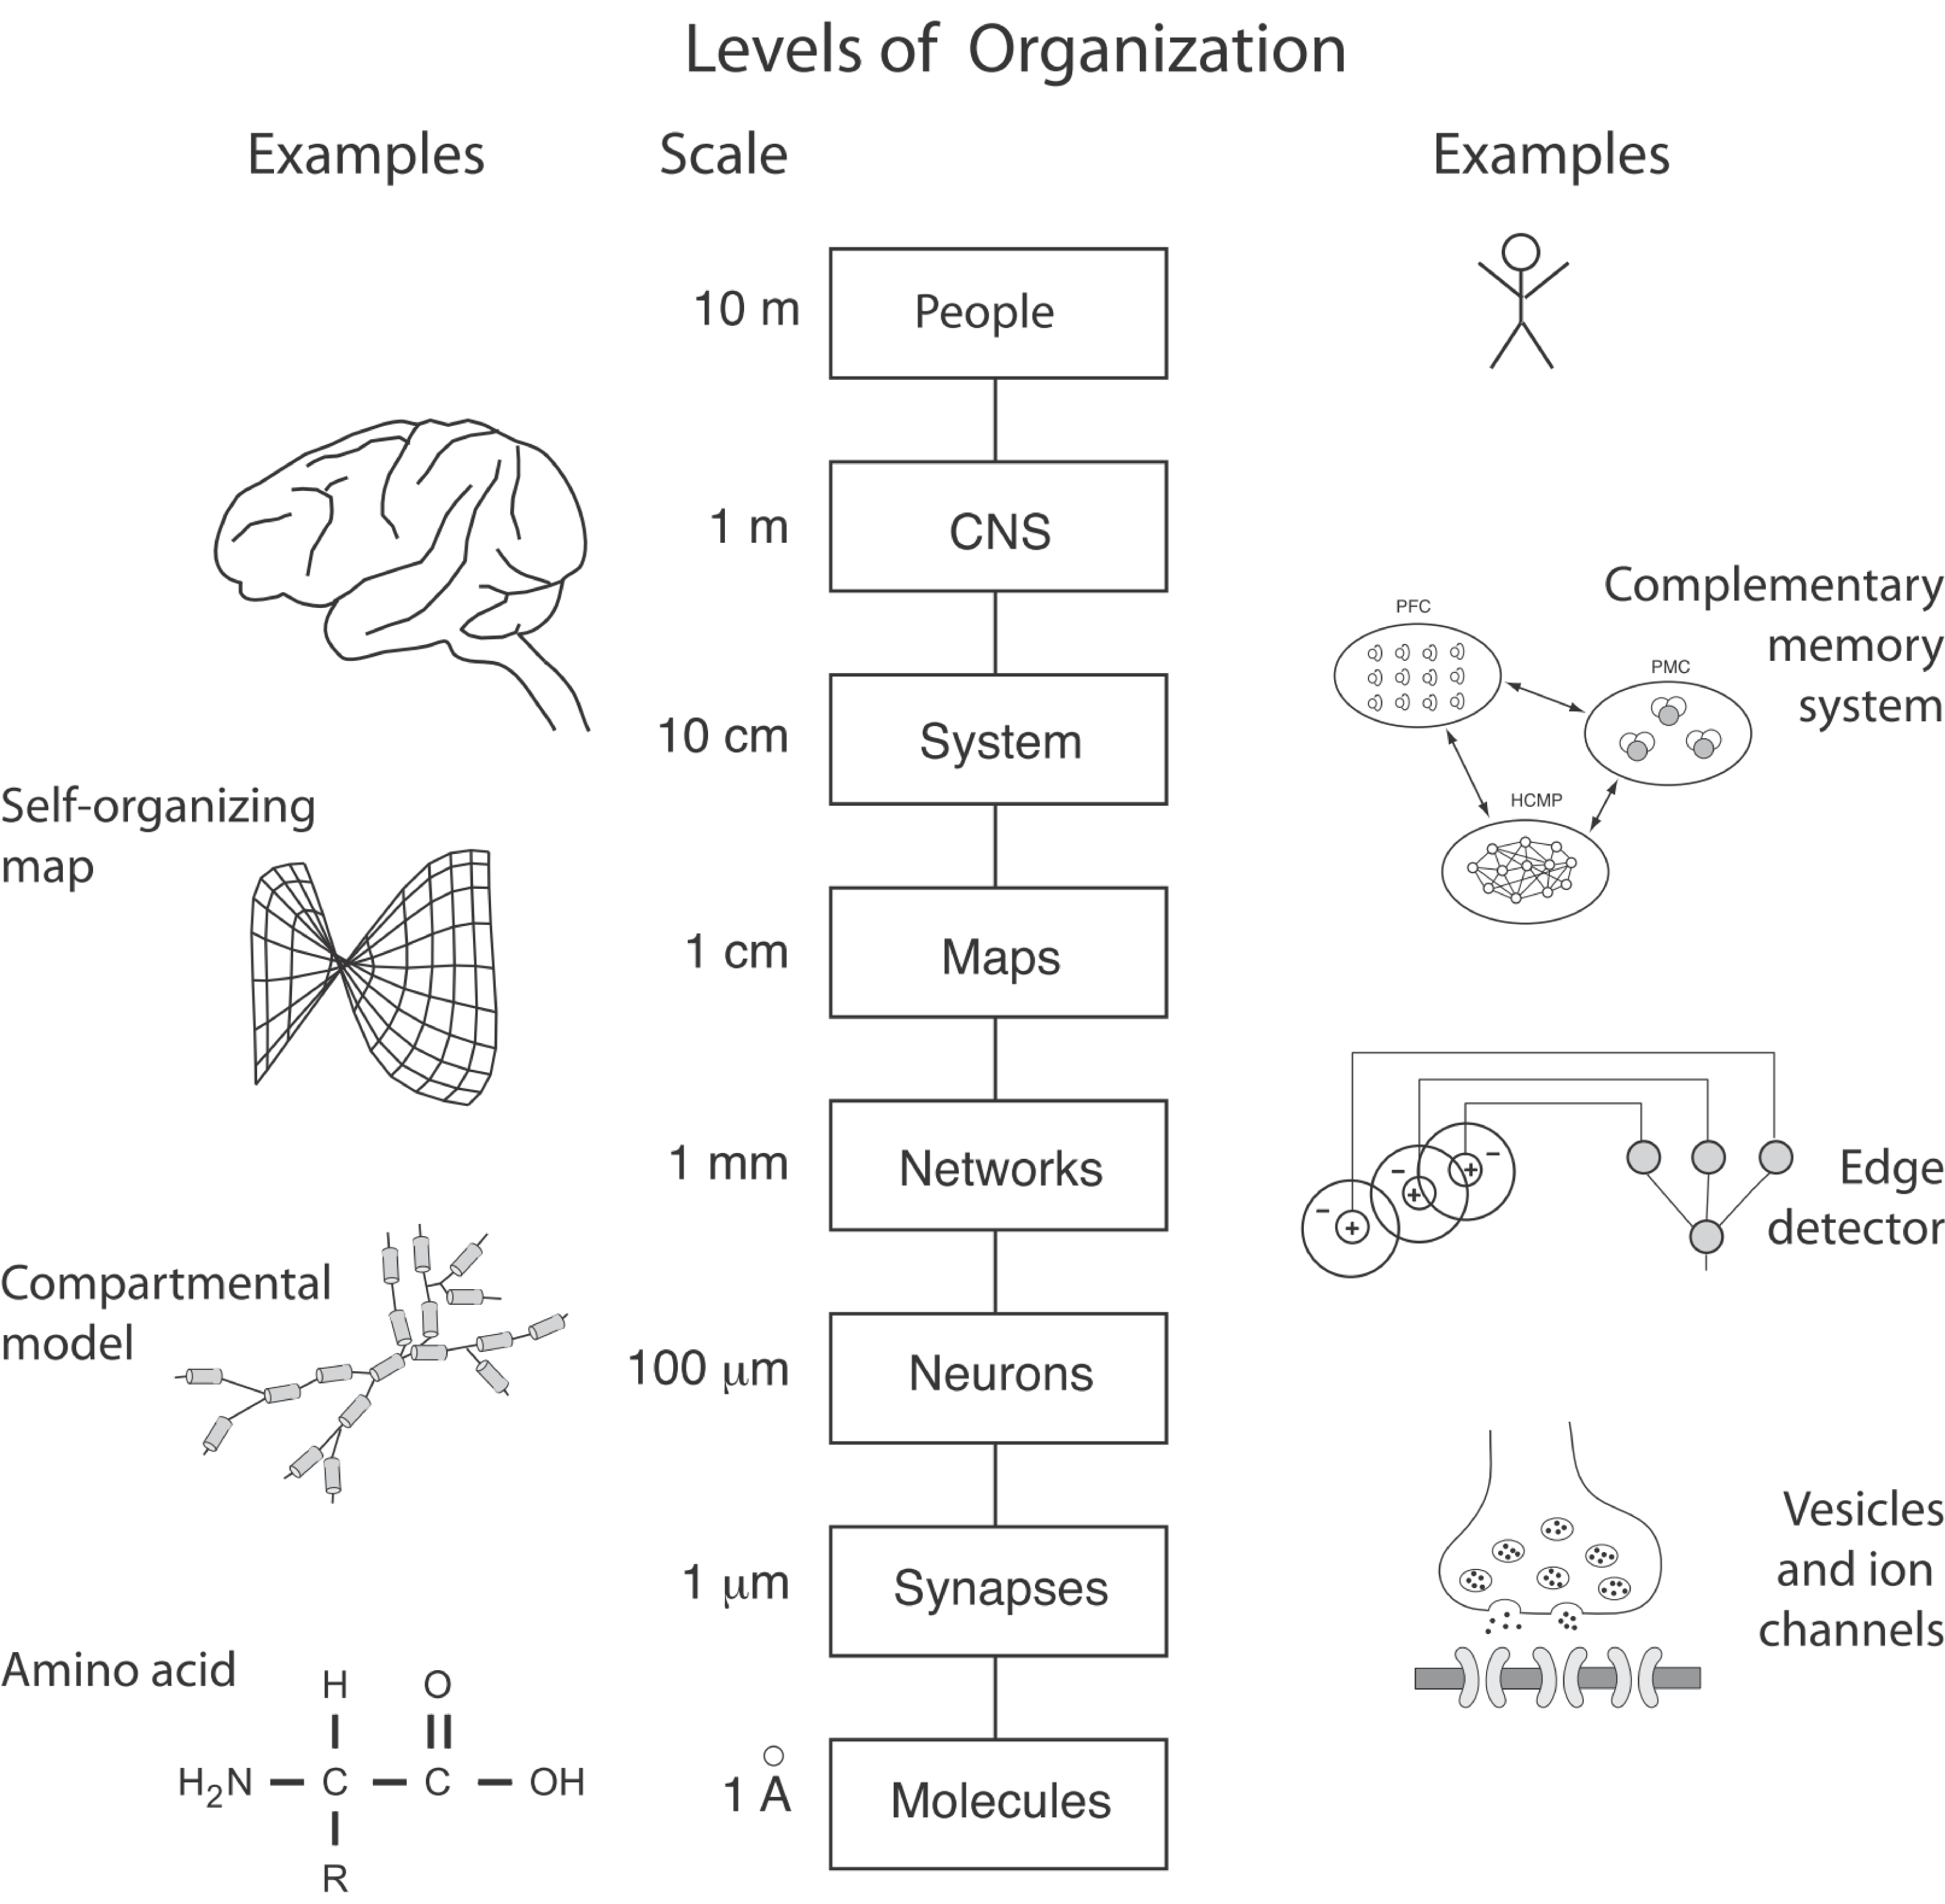
\includegraphics[width=\columnwidth]{graphics/levels.png}
		\caption[The levels of organisation in the \ac{CNS}]{\textbf{The levels of organisation in the \ac{CNS}}. Each level can be modelled in more or less detailed as required. (used with permission of Prof. Trappenberg \cite{Trappenberg2009}).} 
		\label{fig:levels}
\end{figure}


According to the diagram in figure \ref{fig:levels} and the scales, the research reported in this thesis covers the ``Neurons'' level. 

\subsection{Lapicque's integrate-and-fire model}

One of the earliest models of a neuron was in 1907 by Louis Lapicque. Lapicque's model describes what he observed in experiments with frogs. The mechanisms responsible for neuronal action potentials were unknown, and thus Lapicque's model was very simple. Despite the lack of detailed knowledge, Lapicque's model is still the basis of many models that are widely used today \cite{Abbott1999}. Lapicque postulated that nerve membranes were semi-permeable, polarisable membranes and could therefore be modelled as a capacitor with a leak. He compared the data obtained from his frog experiments with both an RC-circuit (a circuit with a resistor and a capacitor in parallel, fig \ref{fig:lapicque}) and a heuristic law of excitability \cite{Brunel2007}.

\begin{figure}[H]
	\centering
		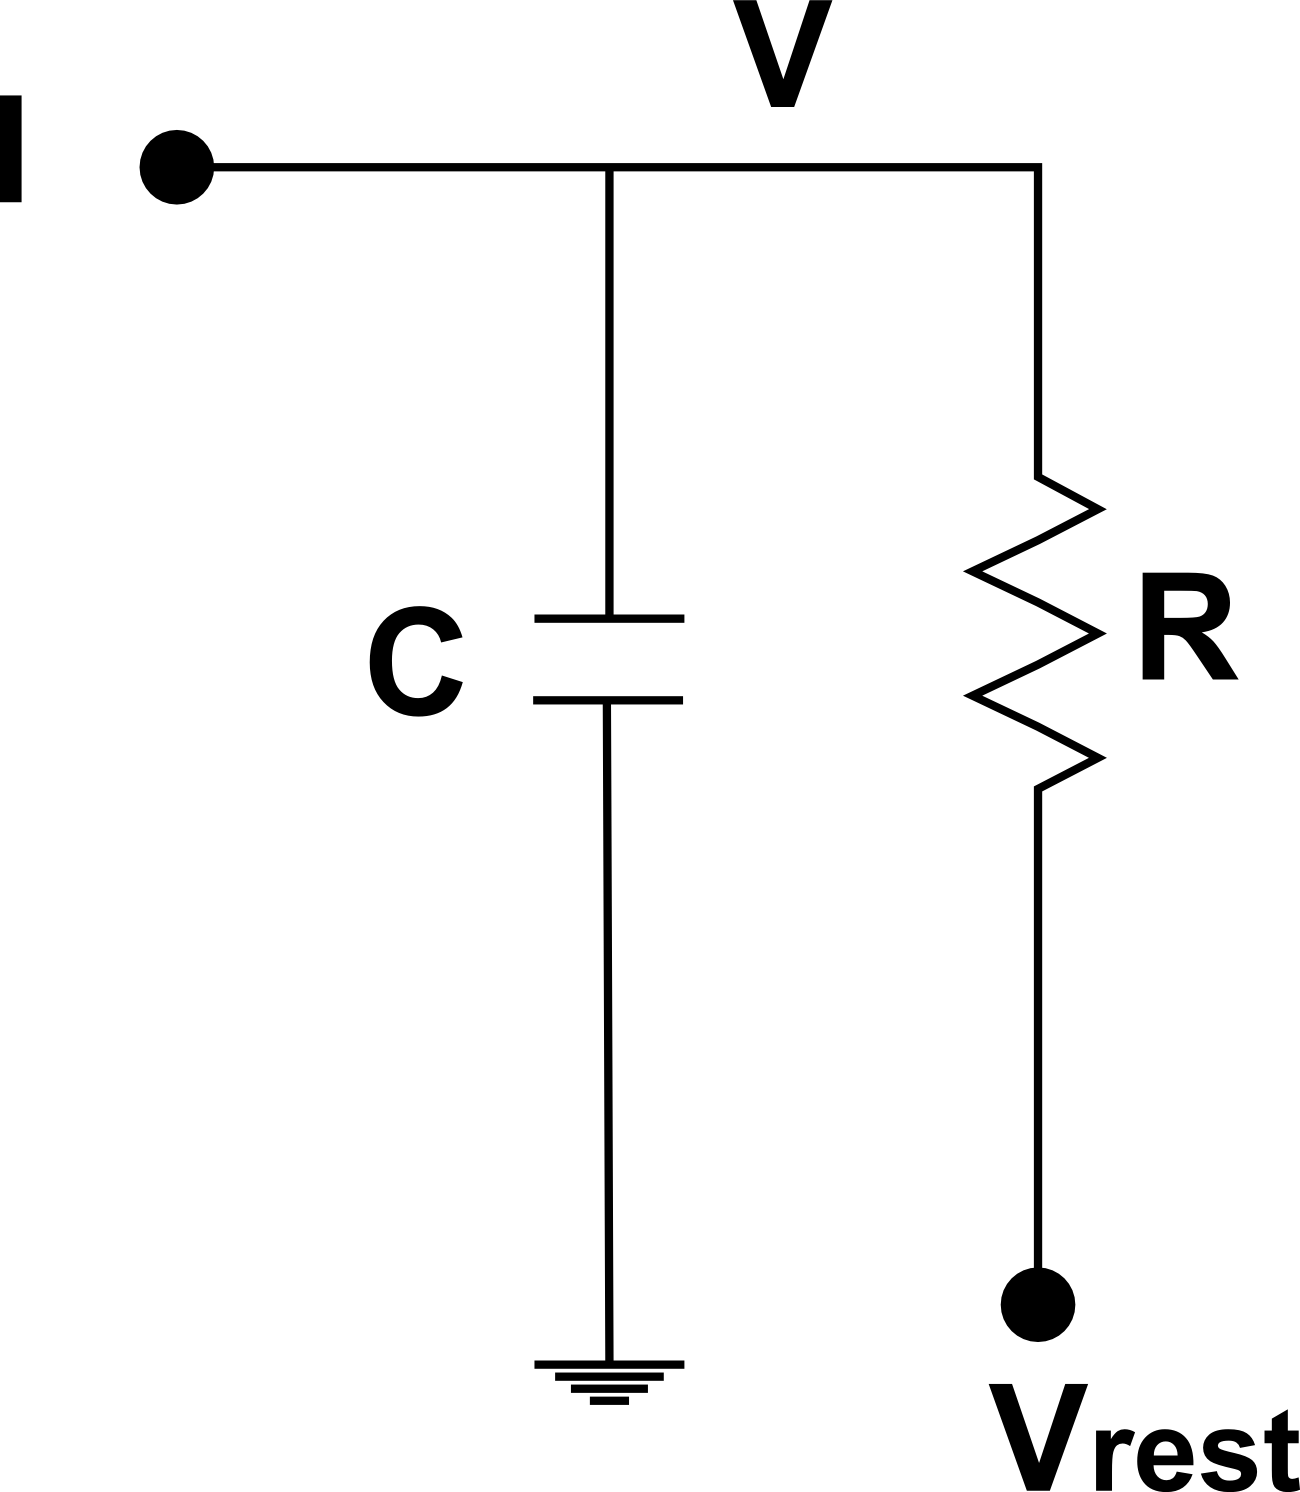
\includegraphics[width=4cm]{graphics/lapicque.png}
		\caption[Lapicque's model]{\textbf{Lapicque's model.} Lapicque's model was based on an RC-circuit. C is the membrane capacitance, R is the membrane resistance, V is the membrane potential, $V_{rest}$ is the resting membrane potential and I is an injected current.}
		\label{fig:lapicque}
\end{figure}

This model can be expressed as the time derivative of the law of capacitance, $Q=CV$. A neuron represented in time would thus be:

\begin{equation}
\label{eq:lapicque}
I(t)=C_{m}\frac{dV_{m}(t)}{dt}
\end{equation}

\subsection{The leaky integrate-and-fire-model}

An improvement on the integrate-and-fire model is the ``leaky integrate-and-fire'' model. This model adds a leak resistance in parallel to the capacitance, which reflects the diffusion of ions through the cell membrane. This model neuron will only fire when the excitatory input is strong enough to overcome the leak (\ref{eq:leaky}).

\begin{equation}
\label{eq:leaky}
I(t)-\frac{V_{m}(t)}{R_{m}}=C_{m}\frac{dV_{m}(t)}{dt}
\end{equation}

The leaky integrate-and-fire model is also known as the ``passive integrate-and-fire'' model because in its simplistic form, all active membrane conductances and synaptic inputs are ignored and the entire membrane is modelled as a single passive leakage term \cite{Dayan2001} %page 164

Semi-permeability of cell membranes is the result of embedded ion channels and pumps. These channels and pumps allow different concentrations of ions to be maintained inside and outside the cell which, in turn, result in an electrical potential existing across the membrane \cite{Sterratt2011}. 

%note {If we don't care about the biomechanical mechanisms, but just want to describe the action potential as a standard pulse then }
\subsection{Hodgkin-Huxley Model}
\label{sec:hogkin_huxley_model}

In 1952 Hodgkin and Huxley described the membrane current in the squid giant axon as an electrical circuit (Fig. \ref{fig:circuit}) and produced a set of differential equations which modelled the ionic currents across the membrane of excitable cells. These equations are still in use today \cite{Hodgkin1952, Hodgkin1952a, Hodgkin1952b, Hodgkin1952c, Hodgkin1952d}. Their work was a breakthrough in the understanding of nerve excitation. The equations in these papers provided only for potassium ion, sodium ion and leak currents. However, the same equations can be used to expand the model to include other currents and as such still serve as the basis of most neuronal models. These models are also known as conductance-based models.

\begin{figure}[H]
	\centering
		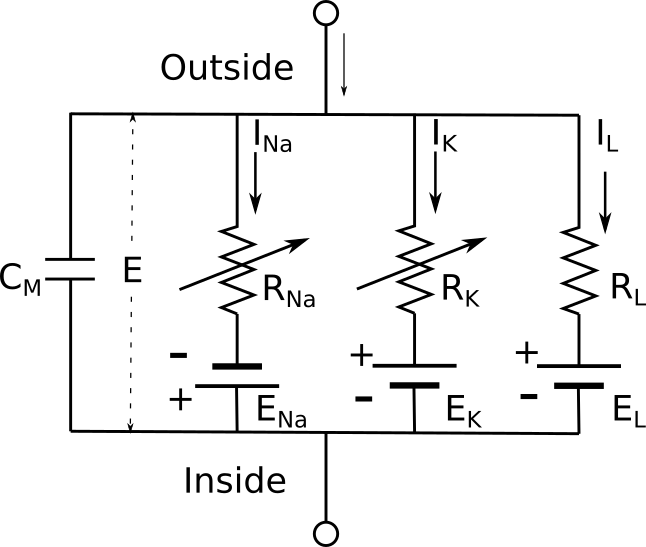
\includegraphics[width=\columnwidth]{graphics/HodgkinHuxley.png}
		\caption[The membrane as an electrical circuit.]{\textbf{The membrane as an electrical circuit.} Hodgkin-Huxey described the membrane current in the squid giant axon as an electrical circuit. \cite{Hodgkin1952a}}
		\label{fig:circuit}
\end{figure}

%See CNN2a.pdf
%Beckerman2005 page 467
Action potentials are the result of joint action by fast-acting sodium channels and delayed-acting potassium channels \cite{Beckerman2005}.
Sodium (Na\textsuperscript{+}) channels can be in any of a number of states, depending on the channel's internal activation, inactivation or deactivation state and whether it is open or closed. The channel only allows Na\textsuperscript{+} to move through when it is both open and activated. Potassium channels have only two states, open or closed. The channels responsible for ``leak currents'' are open all the time and are mostly responsible for the resting membrane potential. The leak current is mostly made up of chloride ions \cite{Hodgkin1952a}. The sodium and potassium channels are also ion specific. However, these channels are voltage dependent, meaning that the probability of them being open or closed depends on the voltage across the cell membrane. In figure \ref{fig:circuit}, this voltage dependency is indicated by the symbol for a variable resistor (a resistor with an arrow through it). 

The mathematical equation for the electrical circuit is given by:

\begin{equation}
\label{eq:membrane_current}
I=C_{M}\frac{dV_{m}}{dt} + I_{int}
\end{equation}

where: 

$I$ is the total membrane current.

$C$ is the membrane capacitance.

$I_{int}$ the sum of the intrinsic and modulatory ionic currents.

$V_{m}$ is the membrane potential.

$t$ is time.



Voltage gated sodium channels in the cell membrane are responsible for the depolarising phase that eventually leads to action potentials. Voltage-gated potassium channels, on the other hand, are crucial for hyperpolarisation to return the cell to a resting state \cite{Lodish2000}.

%\cite{Buchholtz1992}

In the Hodgkin-Huxley model, each of the voltage gated sodium channels is assumed to have two gates: the 'm' and the 'h' gate. For the channel to be open, both gates have to be in an open state. The channel is in a deactivated state if the m channel is closed or an inactivated state if the h channel is closed. When both gates are open the gate is activated. The states of the gates are described in the Hodgkin-Huxley equations by:

\begin{equation}
\label{eq:activationcurve}
I = g_{ion}m^{p}_{ion}h^{q}_{ion}(V - E_{ion})
\end{equation}

As given, this equation (Eq: \ref{eq:activationcurve}) is generic and can be used for all ionic conductances. The maximal conductance of the channel is $g$, while $m$ and $h$ are the fractions of activation and inactivation gates in the open state, and $p$ and $q$ are the number of independent gates per channel. $V$ is the displacement of the membrane potential from its resting value and $E_{ion}$ is the reversal potential that corresponds to the specific ion \cite{Buchholtz1992, Hodgkin1952a, Willms1999, Soto-Trevino2005}.

The Hodgkin-Huxley model of an excitable cell is summarised in four differential equations:

\begin{equation}
\label{eq:HH}
I = C_{m}\frac{d V_{m}}{dt}  + {g}_{K}n^{4}(V_{m} - V_{K}) + {g}_{Na}m^{3}h(V_m - V_{Na}) + g_{l}(V_{m} - V_{l})
\end{equation}
\begin{equation}
\frac{dn}{dt} = \frac{-(n-n_{\infty}(V)) }{ \tau_{n}(V)}
\end{equation}
\begin{equation}
\frac{dm}{dt} = \frac{-(m-m_{\infty}(V)) }{ \tau_{m}(V)}
\end{equation}
\begin{equation}
\frac{dh}{dt} = \frac{-(h-h_{\infty}(V)) }{ \tau_{h}(V)}
\end{equation}

where:

$I$ is the total membrane current,

$C_{m}$ is the membrane capacitance,

$V_{m}$ is the membrane potential,

$t$ is time,

$g_{K}$, $g_{Na}$, $g_{l}$ are the ionic conductances for potassium (K), sodium (Na) and leakage (l) respectively. 

$\alpha$ and $\beta$ are rate constants that vary with voltage but not with time.

The reversal potential for each current can be calculated by using the Nernst equation (Eq. \ref{eq:Nernst})


\begin{equation}
\label{eq:Nernst}
E = \frac{RT}{zF}ln\frac{[ion]_{extracellular}}{[ion]_{intracellular}}
\end{equation}

where:

$E$ is the membrane potential in volts,

$R$ is the ideal gas constant of 8.3144621 $\frac{J}{mol K}$,

$T$ is the temperature in Kelvin,

$z$ is valence of the ion,

$F$ is Faraday's constant for which the currently accepted value is $9.64853399 x 10^{4}C mol^{-1}$,

and $[ion]_{extracellular}$ and $[ion]_{intracellular}$ are the intra- and extracellular ion concentrations respectively in moles per cubic meter.

However, to take into account all of the ions that are permeant through a cell membrane the Goldman-Hodgkin-Katz equation is used:

\begin{equation}\label{eq:GHK}
E_{m} = \frac{RT}{F}ln\frac{P_{Na^{+}}[Na^{+}]_{out}+P_{K^{+}}[K^{+}]_{out}+P_{Cl^{-}}[Cl^{-}] _{in}}{P_{Na^{+}}[Na^{+}]_{in}+P_{K^{+}}[K^{+}]_{in}+P_{Cl^{-}}[Cl^{-}]_{out}}
\end{equation}

Various researchers have based models on the Hodgkin-Huxley model to simplify or adapt the models for specific purposes. Some well-known models the Morris-Lecar \cite{Morris1981} model, FitzHugh-Nagumo \cite{Fitzhugh1961, Nagumo1962} model and the Hindmarsh-Rose model.

\subsection{Multi-compartmental models}
The aforementioned models describe the membrane potential over an entire neuron with a single variable. Membrane and morphological properties vary along the length of an axon resulting in varying membrane potentials over the surface of the neuron \cite{Dayan2001, Sterratt2011}. The effect of the varying membrane potentials and associated complexities can be reproduced in models by considering a neuron as several connected compartments. Each compartment can be simulated by a Hodgkin-Huxley type model (or any other appropriate type of model) with the compartments connected via conductances \cite{Izhikevich2007}\note{page 43}
\note{Dayan, page219}

\subsection{Existing pyloric \ac{CPG} neuron models from literature}
Table \ref{tab:models} lists models of pyloric \ac{CPG} neurons from crustacean that can be found in literature. The table shows the journal reference, the number of neurons that were modelled and the equations that were used. The model with the most number of neurons was the Gutierrez model. The purpose of this model was to illustrate circuit switching using network motifs that are found in the \ac{STG} network. The neurons were modelled as single compartments and using the Morris-Lecar two-dimensional reduced excitation model. Neurons in this model do not reflect physiological properties of the biological neurons (eg. \ac{PD} and \ac{LP} are modelled using the same equations in anti-phase) \cite{Gutierrez2013}.

\begin{table}[H]
	\centering
	\footnotesize
	\caption[\ac{STG} model list]{\textbf{\ac{STG} model list.} A list of published \ac{STG} models by various researchers, showing the number of neurons simulated and the equations used in the model}
	\label{tab:models}
	\begin{tabular}{l l c l l}	
		\textbf{Paper} & \textbf{Neurons} &  \textbf{\#}  & Equations & \textbf{Notes}\\ \hline
		Buchholz 1992 \cite{Buchholtz1992} & LP & 1 & Hodgkin-Huxley & \\
		Epstein 1990 \cite{Epstein1990} & unidentified & 1 & Hodgkin-Huxley & Three models of  \\
		& & & & individual neurons\\
		Golowasch 1992 \cite{Golowasch1992} & LP & 1 & Hodgkin-Huxley & \\ 
		Prinz 2003 \cite{Prinz2003a} & PD & 1 & Hodgkin-Huxley & Database of 1.7 \\
		& & & & million \\
		& & & & single-compartment \\
		& & & & models\\
		
		Abbot 1991 \cite{Abbott1991} & AB, PD & 2 &  FitzHugh-Nagumo & \\
		Golowasch 1999 \cite{Golowasch1999a} & AB/PD, PY & 2 & Hodgkin-Huxley & AB/PD modelled as \\
		& & & & one\\
		Soto-Trevino & AB, PD & 2 & Hodgkin-Huxley & \\
		2005 \cite{Soto-Trevino2005} & & & & \\
		
		Hartline 1979 \cite{Hartline1979} & AB/PD, & 3 &  & AB/PD modelled as\\
		&  LP, PY & & & one\\
		Warshaw 1976 \cite{Warshaw1976} & LP, PD, PY,& 5 & & \\
		& VD, IC & & & \\
		
		Gutierrez 2013 \cite{Gutierrez2013} & IC, LP, & 5 & Morris-Lecar & Illustrating circuit \\
		& LG, PD, Int1 & & & switching\\
	\end{tabular}
\end{table}


Very early models from the Hartline laboratory \cite{Hartline1979, Warshaw1976} also included up to five neurons. These models used Morris-Lecar type equations and were implemented in SNAX, a language for interactive neuronal modelling  and  data  processing \cite{Hartline1976}. SNAX does not seem to be available any more and unfortunately the old journal articles could not be obtained to learn more about the language. 


Note that the Morris-Lecar model is a simplified version of the Hodgkin-Huxley model which, for example, does not capture the details of spiking activity in neurons.  With such a configuration it is not possible to model the differential modulation which occurs when \ac{STG} neurons are exposed to \ac{DA}.

\subsection{How models are created}
The models discussed are expressed as differential equations. These systems are non-linear and cannot be solved analytically. It is possible, though, to use numeric methods. 

An interesting anecdote from the pen of Alan Hodgkin, makes us appreciate the general availability of computers today:

\textit{``Finally there was the difficulty of computing the action potentials from the equations which we had developed. We had settled all the equations and constants by March 1951 and hoped to get these solved on the Cambridge University Computer. However, before anything could be done we learnt that the computer would be off the air for 6 months or so while it underwent a major modification. Andrew Huxley got us out of that difficulty by solving the differential equations numerically using a hand-operated Brunsviga. The propagated action potential took about three weeks to complete and must have been an enormous labour for Andrew. But it was exciting to see it come out with the right shape and velocity and we began to feel that we had not wasted the many months that we had spent in analysing records.''} \cite{Hodgkin1976}

Using MATLAB$^{\copyright}$ on an i5 laptop with 6 gigabytes of RAM and a very simple implementation of the Hodgkin-Huxley model (Appendix \ref{app:HH}), it now takes approximately 0.194440 seconds to produce the graph (Fig. \ref{fig:hh_curve}) that took Andrew Huxley three weeks with the use of the Brunsviga calculator (Fig \ref{fig:brunsviga}).

\begin{figure}[H]
	\centering
		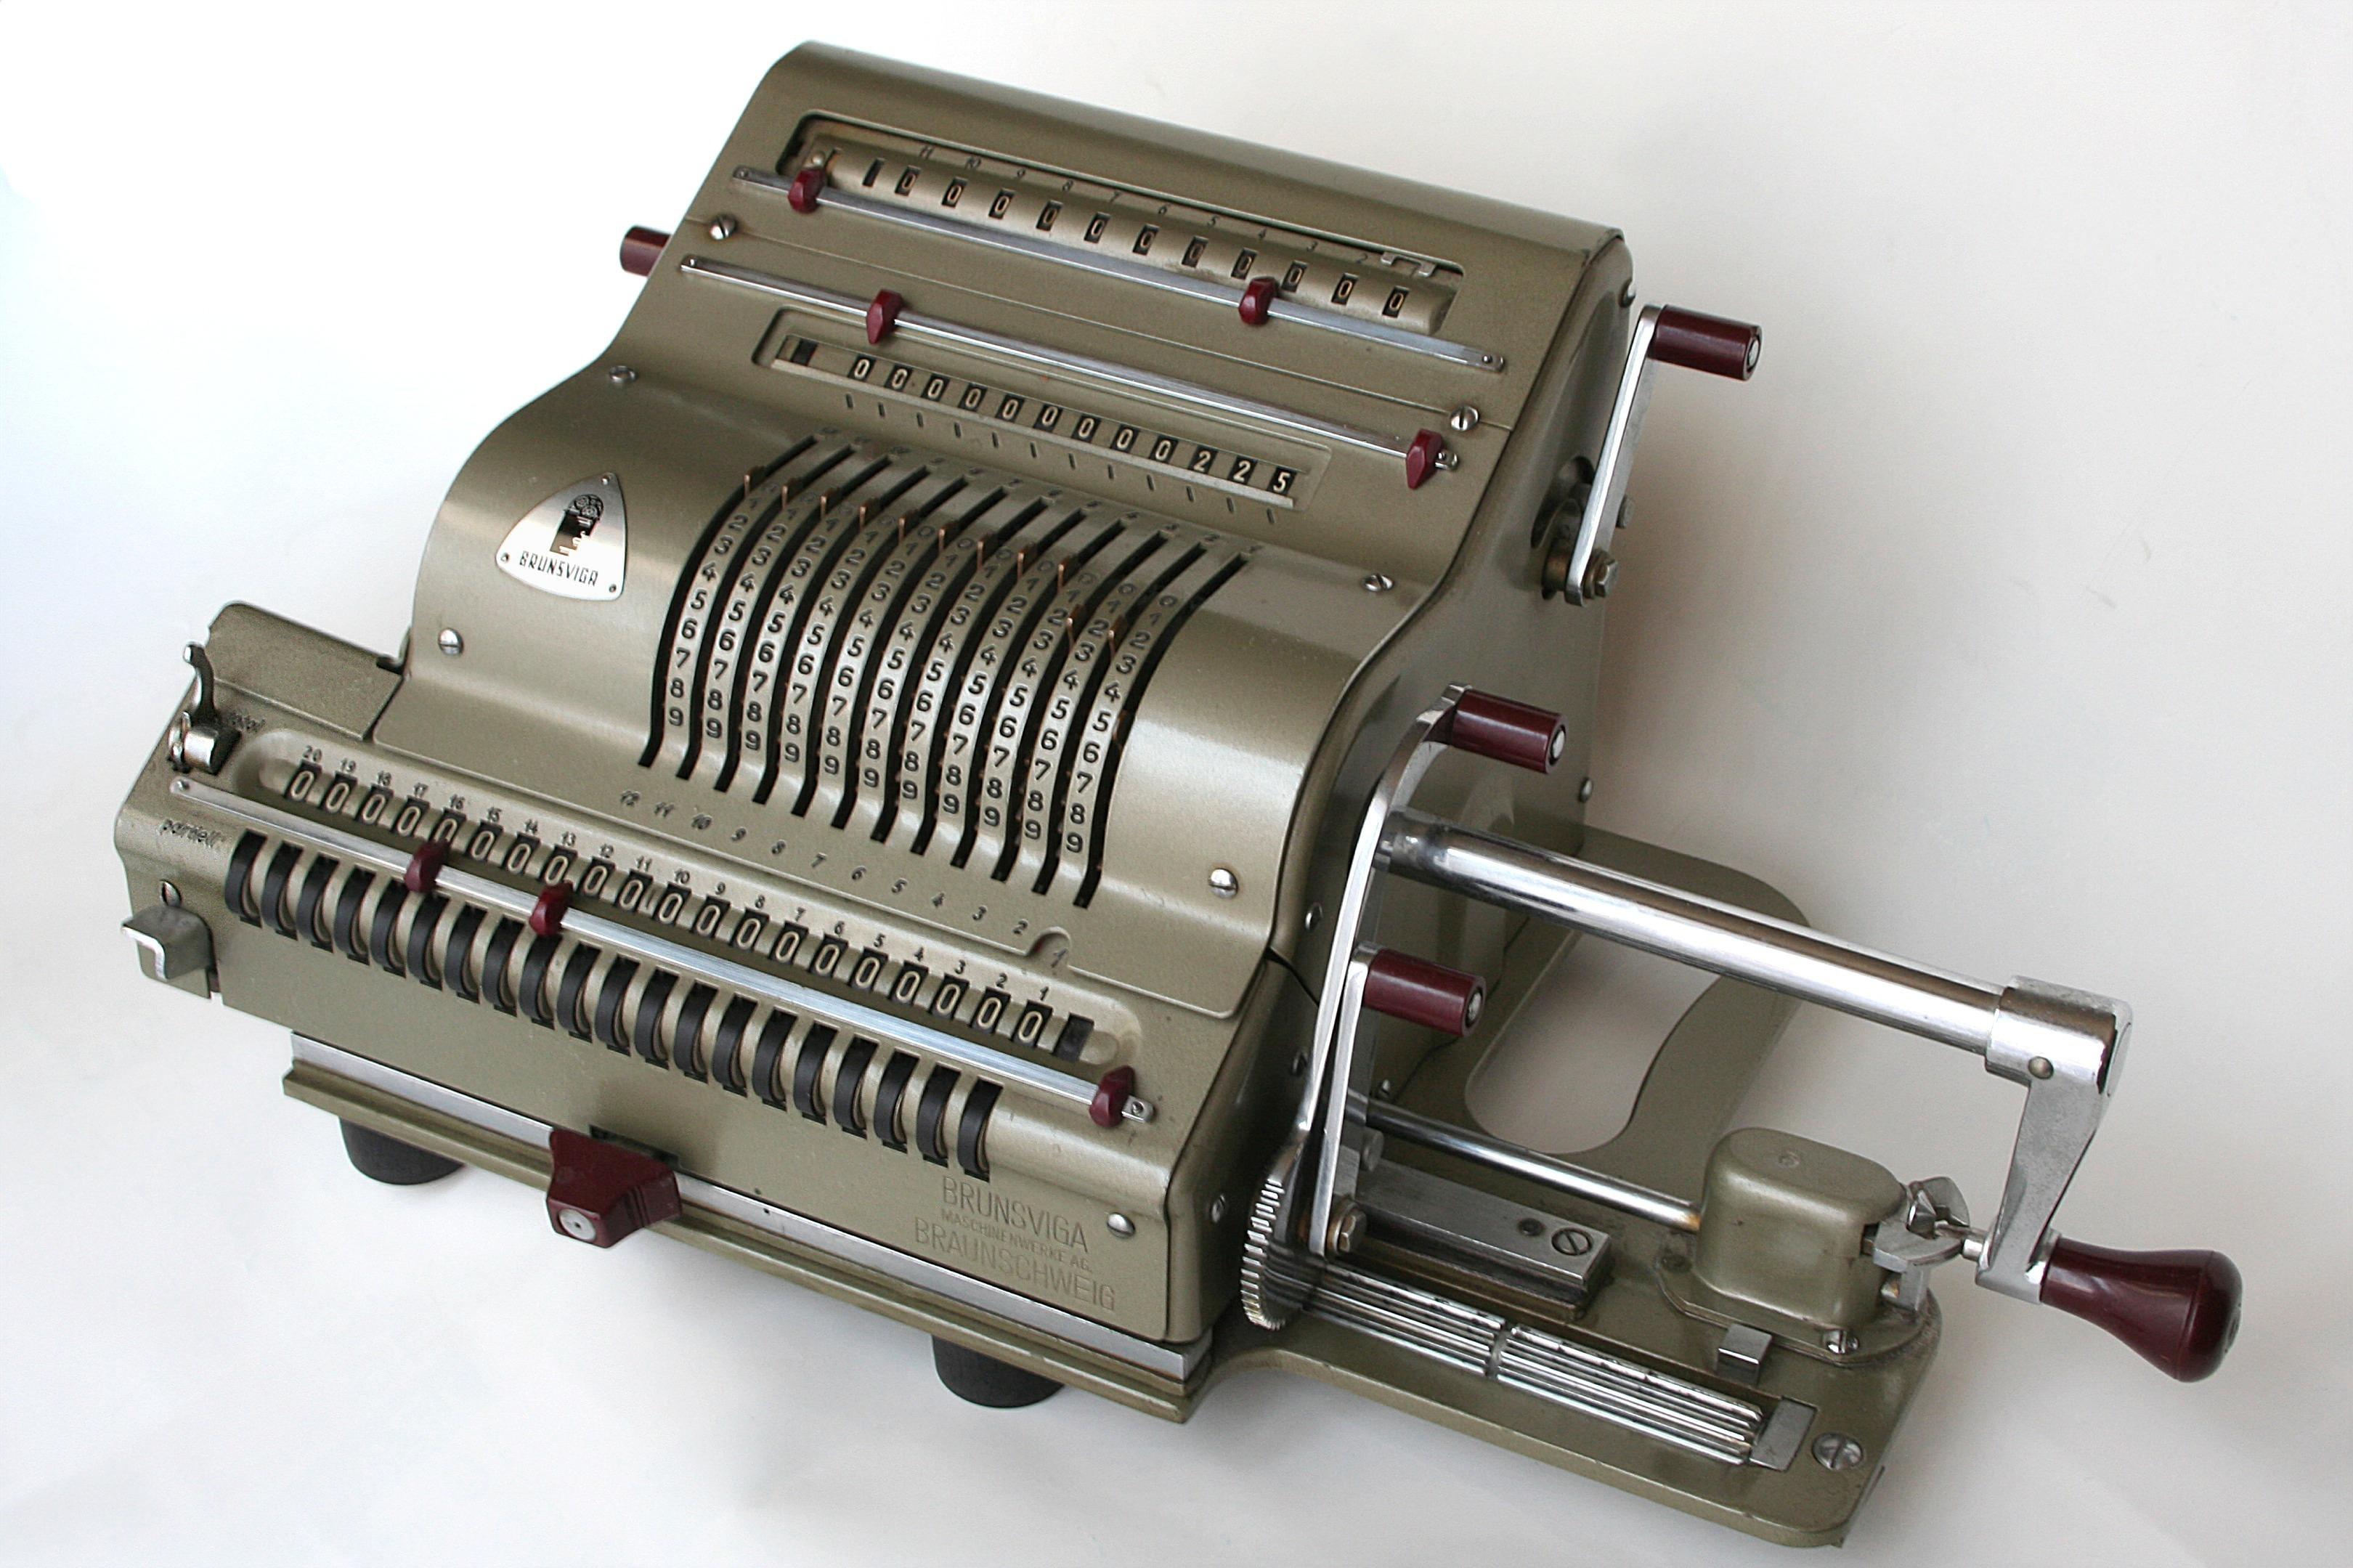
\includegraphics[width=9cm]{graphics/Brunsviga.jpg}
		\caption[A Brunsviga hand-operated calculator]{\textbf{A Brunsviga hand-operated calculator.} A Brunsviga hand-operated calculator such as was used by Andrew Huxley in 1951. (Image by Lothar Spurzem (Spurzem) [CC BY-SA 2.0 de, \url{http://creativecommons.org/licenses/by-sa/2.0/de/deed.en}], Wikimedia Commons)} 
		\label{fig:brunsviga}

		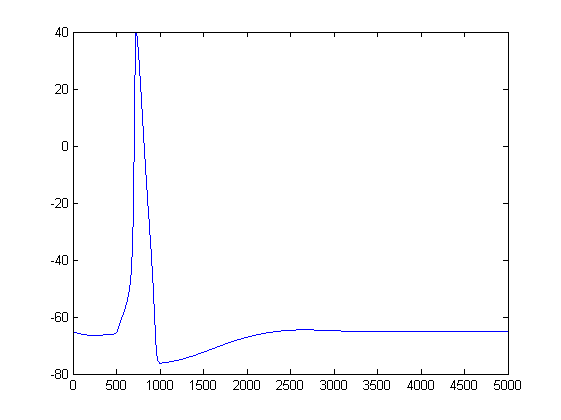
\includegraphics[width=9cm]{graphics/HH_curve.png}
		\caption[An action potential curve]{\textbf{An action potential curve}. A curve produced in 0.194440 seconds with the Hodgkin-Huxley equations using MATLAB$^{\copyright}$.} 
		\label{fig:hh_curve}
\end{figure}

By Lothar Spurzem (Spurzem) (Created by Spurzem.) [CC BY-SA 2.0 de (http://creativecommons.org/licenses/by-sa/2.0/de/deed.en)], Wikimedia Commons

In this day and age and for the purpose of this research it would not be unreasonable to take the availability and use of computers as a given. Thus, the history and details of numerical solvers will not be discussed but rather the software and choices of numerical solvers implemented in the software will be considered. Various numerical solvers are available and it is up to the researchers to select an appropriate solver based on the nature of the equations to be used.

With regards to software there are various commercial and open source packages available such as MATLAB from MathWorks$^{\copyright}$\footnote{\url{https://uk.mathworks.com/products/matlab/}}, GNU Octave\footnote{\url{https://gnu.org/software/octave/}} (an open source product, mostly compatible to MATLAB) and R\footnote{\url{http://www.r-project.org/}} which is also open source. 

There are also software available specifically for neuron simulation such as NEURON\footnote{\url{http://www.neuron.yale.edu/neuron/}} and the GENESIS\footnote{\url{http://genesis-sim.org/}} (GEneral NEural Simulation System) simulator. These simulators have built-in numerical solvers and in some cases the user might be offered a selection of solvers to choose from.

The stiffness of the equations of the selected model is an important determinant in the selection of the appropriate software and numerical solver to be used. ``Stiffness'' arises when one has to deal with more than one first-order differential equation where some dependent variables are changing based on two or more independent variables that have very different scales \cite{Press1992}.\note{page 734, section c16-6}

\note{Curtiss1952, ode45berkley}

In the case of the Hodgkin-Huxley model there are slow components and fast components. The equations are stiff because of the interactions between the membrane potential and the three conductance variables \cite{Chance1981}. Thus a numerical solver that can cope with this ``stiffness'' in the equations need to be selected.

Typically, for models derived from the Hodgkin-Huxley model, a fourth-order Runge-Kutta method with predictions is used (Runge-Kutta(4,5)). Predictions are made with an adaptive step-size algorithm.

Another interesting result from the Hodgkin-Huxley studies is the fact that neurons emerged as dynamical systems and can therefore be studied as such. 

The Hodgkin-Huxley model is a four-dimensional dynamical system of ordinary differential equations governing the evolution of four state variables, $V$, $n$, $m$ and $h$ \cite{Izhikevich2007}. The model exhibits bi-stability between equilibrium and limit cycle attractors. If a constant current is injected that is below the threshold where tonic firing takes place, the system will go to a fixed point. When a higher current is injected, the fixed point becomes unstable and solutions converge to a stable periodic trajectory which is known as a limit cycle (figure \ref{fig:limitcycle}) \cite{Fitzhugh1960, Meunier2001}.

\begin{figure}[H]
	\centering
		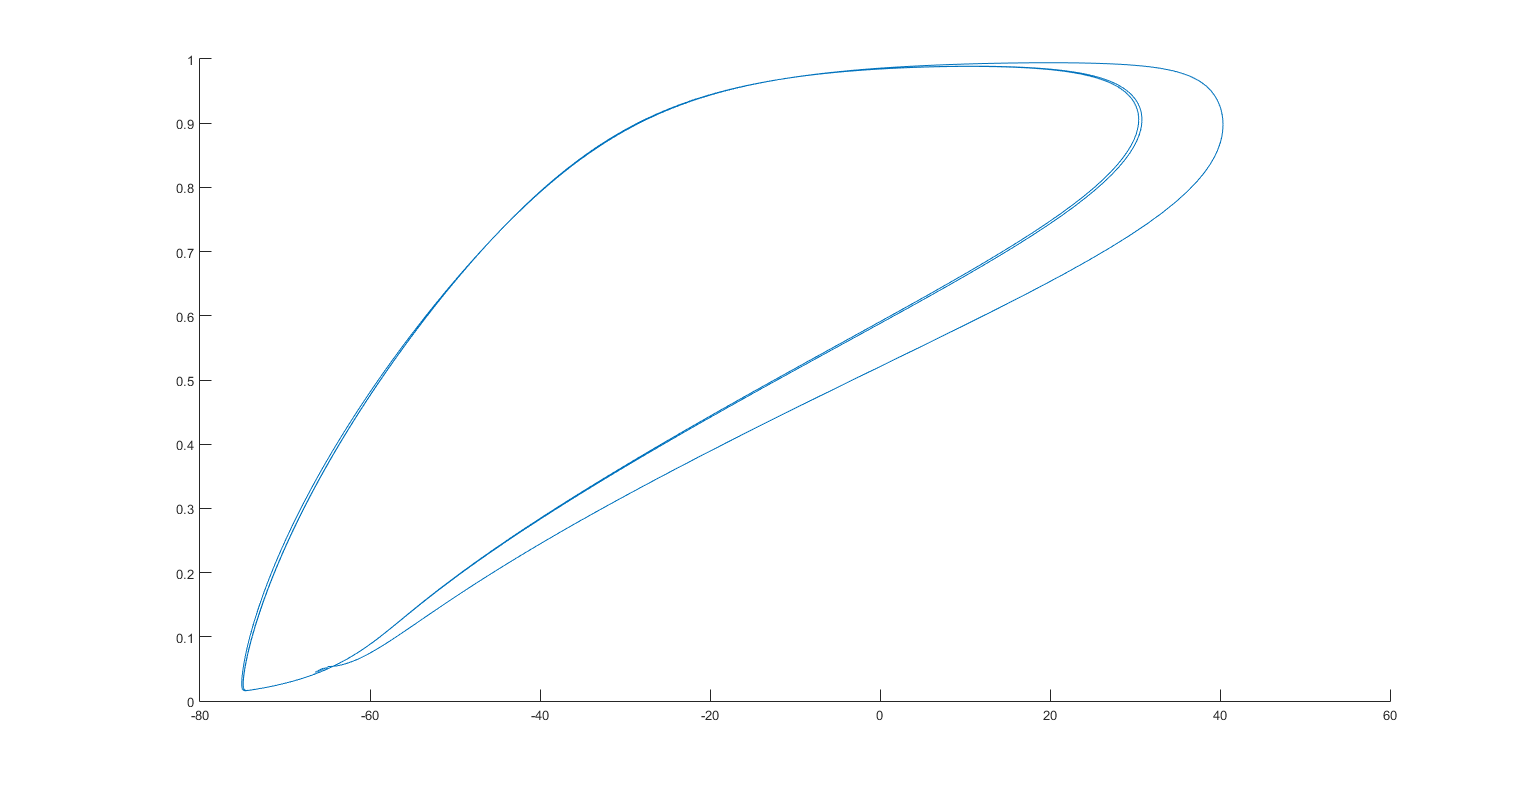
\includegraphics[width=\columnwidth]{graphics/limitcycle.png}
		\caption[Limit cycle]{\textbf{Limit cycle.} Using the model from appendix \ref{app:HH}, this limit cycle was produced by plotting $m$ against $v$.}
		\label{fig:limitcycle}
\end{figure}

\note{\url{https://books.google.co.uk/books?id=w8Nxnr47690C&pg=PA371&lpg=PA371&dq=hodgkin+huxley+dynamical+system+fixed+attractor&source=bl&ots=akbF-Z3f6E&sig=kELxQwL79QkxHeMkERwcmoUbPaQ&hl=en&sa=X&ei=uMIvVfnyBMHiaMGdgPAB&ved=0CDwQ6AEwAw#v=onepage&q=hodgkin\%20huxley\%20dynamical\%20system\%20fixed\%20attractor&f=false}}
\note{system in permanent flux - Belousov Zhabotinsky reaction
	
	when the neuron is spiking you need a limit cycle attractor and not a fixed point attractor
	Describe that if you have these equations then how does the system works . say something about the equilibrium point being stable or unstable . When it is stable it is a fixed point attractor when not then talk about other attractors such as limit cycles such as strange (chaotic) attractor which won't discuss.
	Paper not finished because did not do enough temporal averaging
}
\note{
	http://stsutsui.com/projects/hh.html}
\subsection{Finding Parameters}
A vital aspect of computational modelling is finding appropriate values for model parameters. The values could be based on measurements taken during experiments, but are often estimates or even complete guesses \cite{Sterratt2011}.

In the Hodgkin-Huxley based models there is requirement for conductance values ($g$). These values are usually experimentally measured but are highly variable \cite{Golowasch1999,Zhao2012}. Prinz, for instance, computationally generated 20,250,000 model networks from combinations of a three neuron circuit varying the synaptic strengths and neuron properties. The circuit was based on the pyloric \ac{CPG} of \species{H. americanus}. Of these model  4,047,375, 20\%, produced pyloric-like behaviour, confirming that similar network activity can be produced from disparate circuit parameters \cite{Prinz2004a}.

It has also been shown, in the pyloric neurons of the crustacean \ac{STG}, that ionic conductances are expressed in a correlated fashion \cite{Temporal2012} and that these correlations contribute to the invariance of neuron activity and spiking frequencies \cite{Zhao2012}. 
\note{\cite{Hodgkin1952d,Soto-Trevino2005}}
\note{Bumbaugh-thesis}
\note{stiffness: mascagni_sherman.pdf page 32}

% words 6250

This background section is by no means comprehensive. Each of the sections covered justifies research in its own right and is the subject of several books, articles and research groups. The nature of this research is such that it requires an interdisciplinary approach. Continuous progress in technology also means that knowledge and skills of all the contributory fields need to be kept up to date. For instance, progress made in optogenetics might soon make it an option for recording neural activity in the \ac{STG}. The background given, will hopefully serve to put the research question and the technical requirements into perspective.

